% ==============================================================================
% DASK 2026 - Yarışma Soruları
% İstanbul Finans Merkezi (41.002136°, 29.106832°)
% ==============================================================================
\documentclass[12pt,a4paper]{article}
\usepackage[utf8]{inputenc}
\usepackage[T1]{fontenc}
\usepackage{lmodern}
\usepackage[shorthands=off,turkish]{babel}
\usepackage{geometry}
\usepackage{graphicx}
\usepackage{pgfplots}
\usepgfplotslibrary{fillbetween}
\usepackage{booktabs}
\usepackage{amsmath}
\usepackage{tikz}
\usetikzlibrary{shapes.geometric, positioning, arrows.meta, decorations.pathreplacing}
\usepackage{float}
\usepackage{hyperref}
\usepackage{fancyhdr}
\usepackage{lastpage}
\usepackage{amssymb}
\usepackage{textcomp}
\usepackage{setspace}


% DASK tikz logo için premble ayarları
\usetikzlibrary{svg.path}

% Define the Coca-Cola Red color from the SVG (Hex #D6181F)
\definecolor{CocaColaRed}{HTML}{D6181F}

% Roman rakamları için makro (Türkçe babel uyumlu)
\makeatletter
\newcommand{\RN}[1]{\@Roman{#1}}
\makeatother

\geometry{margin=2.5cm, headheight=14.5pt}
\pgfplotsset{compat=1.18}
\pgfplotsset{
    sciencestyle/.style={
        tick align=inside,
        major tick length=4pt,
        minor tick length=2pt,
        tick style={thin, black},
        axis line style={thin, black},
        xtick pos=both,
        ytick pos=both,
        xticklabel pos=lower,
        yticklabel pos=left,
        grid=major,
        grid style={line width=0.08pt, draw=gray!18},
        tick label style={font=\small},
        label style={font=\small},
        legend style={font=\scriptsize, draw=gray!50, fill=white, fill opacity=0.95, cells={anchor=west}, rounded corners=0.5pt},
        every axis plot/.append style={line width=0.8pt},
    }
}
\setlength{\parindent}{1.5em}

\hypersetup{
    colorlinks=true,
    linkcolor=blue,
    citecolor=blue,
    urlcolor=blue
}

% Header/Footer
\pagestyle{fancy}
\fancyhf{}
\fancyhead[L]{DASK 2026}
\fancyhead[R]{\small İzmir Yüksek Teknoloji Enstitüsü Proje Teklifi}
\fancyfoot[L]{ \small DASK Depreme Dayanıklı Bina Tasarımı Yarışması Proje Teklifi}
\fancyfoot[R]{\thepage/\pageref{LastPage}}
\renewcommand{\headrulewidth}{0.4pt}
\renewcommand{\footrulewidth}{0.4pt}

\begin{document}

% --- KAPAK SAYFASI ---
\hypersetup{pageanchor=false}
\begin{titlepage}
\begin{onehalfspacing}
    \centering
    \vspace*{1cm}
    
    \resizebox{8cm}{!}{

\begin{tikzpicture}
    % The raw SVG coordinates are very large (~15000 units) and "Cartesian" (Y-up).
    % We scale them down by 0.005 to fit the document (~7.5cm width).
    % No negative yscale is needed because TikZ is naturally Y-up.
    \fill[color=CocaColaRed, scale=0.005] svg {
        % Main Script Path
        M8120 15079 c-2794 -163 -5183 -2080 -5950 -4774 -387 -1362 -321
        -2834 187 -4159 636 -1657 1927 -2996 3563 -3696 1221 -522 2601 -661 3905
        -394 1381 284 2624 996 3569 2044 788 875 1325 1936 1560 3085 268 1311 129
        2678 -396 3910 -645 1512 -1855 2743 -3359 3418 -958 430 -2028 627 -3079 566z
        m2543 -1099 l527 -150 418 -210 c229 -115 413 -209 407 -209 -5 0 -463 113
        -1016 252 l-1007 253 -86 -56 c-86 -55 -617 -396 -773 -497 -46 -29 -83 -51
        -83 -49 0 3 37 33 83 68 45 35 262 204 482 374 521 404 494 384 508 379 6 -3
        249 -72 540 -155z m-163 -325 c184 -42 343 -78 353 -81 16 -5 17 -25 17 -236
        0 -180 -3 -229 -12 -226 -7 3 -172 40 -365 84 l-353 79 0 232 c0 182 3 231 13
        228 6 -3 163 -39 347 -80z m-610 -150 l0 -226 -207 -136 c-115 -75 -293 -192
        -398 -261 -104 -68 -195 -127 -202 -129 -11 -4 -13 40 -11 223 l3 229 65 43
        c468 312 727 480 738 481 9 1 12 -50 12 -224z m1710 -115 c212 -44 388 -80
        393 -80 4 0 7 -103 7 -230 0 -135 -4 -230 -9 -230 -18 0 -783 160 -792 166 -5
        3 -9 106 -9 230 0 174 3 224 13 224 7 0 185 -36 397 -80z m-1120 -350 c173
        -39 332 -75 353 -81 l37 -10 0 -229 c0 -127 -1 -230 -2 -230 -2 1 -165 38
        -363 83 l-360 82 -3 232 c-2 184 0 232 10 228 7 -2 155 -36 328 -75z m-590
        -155 l0 -225 -127 -83 c-71 -46 -249 -164 -398 -262 -148 -98 -276 -180 -282
        -182 -10 -4 -13 44 -13 223 l0 229 143 92 c78 51 257 169 397 262 140 93 261
        170 268 170 9 1 12 -50 12 -224z m1662 -104 c183 -38 359 -74 391 -81 l57 -11
        0 -230 c0 -135 -4 -229 -9 -229 -5 0 -43 7 -83 16 -40 8 -214 44 -387 80 -172
        35 -317 67 -322 70 -5 3 -9 106 -9 230 0 186 2 224 14 224 8 0 164 -31 348
        -69z m-1072 -361 c173 -39 332 -75 353 -81 l37 -10 0 -230 0 -229 -22 5 c-13
        3 -176 41 -363 83 l-340 77 -3 232 c-2 184 0 232 10 228 7 -2 155 -36 328 -75z
        m-590 -155 l0 -226 -112 -73 c-100 -64 -506 -331 -644 -422 -28 -19 -54 -34
        -58 -34 -3 0 -6 101 -6 225 l0 225 43 30 c127 89 754 498 765 499 9 1 12 -50
        12 -224z m2190 -955 l0 -1050 770 0 c678 0 770 -2 770 -15 0 -13 -92 -15 -770
        -15 l-770 0 0 -1440 c0 -1433 0 -1440 -20 -1440 -20 0 -20 7 -20 1441 0 1348
        -1 1440 -17 1437 -12 -2 -83 -162 -245 -553 -126 -303 -229 -559 -229 -570 0
        -11 60 -249 134 -530 75 -280 161 -607 192 -725 31 -118 59 -223 61 -233 5
        -16 -15 -17 -357 -15 l-362 3 -12 42 c-7 24 -86 318 -176 655 l-164 612 -6
        -514 c-3 -283 -7 -579 -8 -657 l-1 -143 -356 0 -356 0 4 78 c2 42 8 85 12 95
        18 39 -31 15 -97 -48 -69 -65 -117 -90 -234 -120 -160 -42 -435 -44 -571 -5
        -200 57 -394 211 -465 370 -42 94 -49 140 -54 353 l-5 207 341 0 341 0 0 -115
        c0 -150 13 -210 55 -252 28 -28 40 -33 81 -33 67 0 111 28 120 76 12 66 -1
        196 -26 244 -48 94 -98 141 -295 274 -148 101 -223 165 -295 254 -75 93 -80
        94 -152 24 -27 -26 -48 -44 -48 -41 0 3 16 45 35 94 l34 88 -19 28 c-42 58
        -92 180 -105 256 -18 101 -18 165 0 286 32 212 143 379 324 485 l46 27 -172 3
        c-145 2 -173 5 -173 17 0 13 31 15 209 15 169 0 222 3 273 18 87 24 389 23
        498 -1 49 -11 120 -17 208 -17 l132 0 0 510 c0 313 4 510 9 510 11 0 655 -138
        684 -146 16 -5 17 -35 17 -440 l0 -434 179 0 179 0 18 53 c9 28 18 53 19 55 1
        1 133 -23 294 -53 236 -45 312 -55 397 -55 l104 0 0 1050 c0 1043 0 1050 20
        1050 20 0 20 -7 20 -1050z m-719 891 c79 -17 254 -53 388 -80 133 -28 245 -51
        247 -51 2 0 4 -103 4 -230 0 -126 -3 -230 -7 -230 -14 0 -788 162 -795 167 -5
        2 -8 105 -8 229 0 181 3 224 13 224 8 0 79 -13 158 -29z m-1471 -510 l0 -229
        -405 -266 c-223 -146 -408 -266 -410 -266 -3 0 -5 102 -5 228 l0 227 190 125
        c389 256 625 410 627 410 2 0 3 -103 3 -229z m570 155 c157 -35 311 -70 344
        -77 32 -7 60 -18 62 -24 3 -6 3 -110 2 -231 l-3 -221 -75 17 c-41 10 -187 43
        -325 74 -137 32 -267 62 -287 67 l-38 10 0 230 c0 215 1 230 18 225 9 -3 145
        -34 302 -70z m-1877 -60 c15 -15 16 -109 34 -2524 5 -765 8 -905 20 -909 24
        -9 31 9 35 97 2 69 0 85 -12 85 -8 0 -17 -11 -21 -25 l-7 -25 -1 25 c-1 74 47
        1028 53 1038 13 21 56 14 66 -10 5 -13 19 -166 31 -340 13 -175 27 -318 31
        -318 4 0 10 11 14 24 4 17 11 22 24 19 12 -3 30 8 54 34 19 21 36 33 36 27 0
        -15 -120 -317 -132 -331 -15 -18 -55 -16 -62 3 -11 30 -6 69 14 99 11 17 20
        38 20 48 0 20 -25 23 -37 5 -5 -9 -10 -3 -14 17 -6 25 -7 22 -8 -18 0 -26 -10
        -66 -22 -88 -22 -44 -20 -69 6 -69 13 0 15 -7 11 -27 -3 -16 -8 -122 -12 -236
        -4 -114 -9 -205 -13 -202 -3 4 -10 32 -16 63 -7 40 -15 57 -25 57 -11 0 -14
        -11 -13 -45 3 -69 23 -140 39 -140 10 0 14 -13 14 -47 -1 -127 -59 -1303 -64
        -1312 -13 -20 -56 -12 -65 12 -6 12 -15 836 -21 1902 -7 1034 -13 1881 -14
        1882 -1 1 -32 -499 -69 -1110 -38 -612 -70 -1122 -73 -1134 -5 -29 -41 -40
        -62 -19 -11 11 -17 44 -20 126 -3 61 -7 109 -9 106 -3 -3 -18 -111 -33 -240
        -16 -136 -33 -242 -40 -251 -16 -19 -34 -19 -54 1 -13 13 -16 48 -17 212 -1
        193 -2 187 -33 -328 -17 -289 -35 -531 -39 -537 -11 -17 -42 -16 -56 1 -8 10
        -14 155 -19 503 l-7 488 -24 -285 c-13 -157 -28 -291 -34 -297 -12 -16 -53
        -17 -62 -3 -4 6 -20 507 -36 1113 -16 606 -30 1105 -32 1110 -1 4 -26 -376
        -55 -845 -31 -499 -58 -858 -64 -865 -13 -17 -43 -17 -56 0 -7 8 -15 187 -22
        502 -6 270 -12 504 -13 520 -1 18 -20 -39 -44 -137 l-43 -168 0 -410 0 -410
        -340 0 -340 0 0 148 -1 147 -22 -39 c-43 -75 -113 -161 -162 -198 -81 -62
        -143 -81 -276 -86 -125 -4 -199 9 -267 49 -18 10 -35 19 -38 19 -2 0 -4 -171
        -4 -380 l0 -380 -30 0 c-20 0 -30 -5 -30 -15 0 -12 -18 -15 -105 -15 -87 0
        -105 3 -105 15 0 12 -18 15 -105 15 -87 0 -105 -3 -105 -15 0 -12 -18 -15
        -105 -15 -98 0 -105 1 -105 20 0 17 7 20 45 20 l45 0 0 118 -1 117 -36 -69
        c-50 -93 -117 -159 -200 -199 -66 -31 -72 -32 -203 -32 -117 0 -141 3 -182 22
        -61 28 -128 91 -155 145 -54 108 -53 75 -53 1251 0 1228 -3 1176 73 1290 70
        103 165 147 321 147 172 0 301 -78 398 -239 l28 -46 0 463 0 462 400 0 c393 0
        400 0 400 -20 0 -19 -7 -20 -95 -20 l-95 0 0 -116 0 -115 64 46 c177 126 414
        180 680 156 309 -29 525 -158 631 -376 65 -134 67 -152 72 -655 l5 -455 42
        164 c43 171 57 198 94 175 15 -10 17 -31 20 -160 1 -82 6 -152 10 -156 5 -5
        30 351 57 789 44 712 52 800 68 816 13 13 22 15 36 7 15 -7 21 -25 25 -72 3
        -35 17 -556 31 -1158 14 -602 29 -1113 33 -1135 5 -28 16 63 36 300 16 187 33
        348 38 358 6 12 18 17 36 15 l27 -3 7 -259 c4 -142 9 -260 10 -262 2 -2 19
        268 37 599 34 610 38 647 74 647 36 0 37 -11 37 -639 0 -338 2 -612 4 -610 2
        2 11 64 20 138 9 73 19 138 22 142 9 15 53 10 62 -8 13 -23 11 -54 103 1427
        70 1137 82 1297 96 1308 21 15 28 15 46 -2z m3038 -211 c200 -41 374 -77 387
        -80 l22 -5 0 -230 c0 -127 -3 -230 -7 -229 -5 0 -186 37 -403 82 l-395 82 -3
        228 c-2 217 -2 227 17 227 10 0 182 -34 382 -75z m-1731 -510 l0 -226 -278
        -183 c-400 -264 -513 -337 -529 -343 -11 -4 -13 36 -13 220 l0 226 24 18 c14
        10 105 70 203 135 98 64 268 175 377 247 110 72 203 131 208 131 4 0 8 -101 8
        -225z m1735 -120 c204 -42 378 -78 388 -81 16 -5 17 -25 17 -234 l0 -229 -27
        5 c-16 3 -197 40 -403 83 l-375 77 -3 219 c-1 121 0 225 2 232 3 7 11 11 18 8
        7 -2 180 -38 383 -80z m-8295 -45 c0 -19 -7 -20 -105 -20 -98 0 -105 1 -105
        20 0 19 7 20 105 20 98 0 105 -1 105 -20z m420 0 c0 -19 -7 -20 -105 -20 -98
        0 -105 1 -105 20 0 19 7 20 105 20 98 0 105 -1 105 -20z m418 -2 c3 -16 -7
        -18 -107 -18 -105 0 -111 1 -111 20 0 20 5 21 107 18 93 -3 108 -5 111 -20z
        m412 2 c0 -19 -7 -20 -105 -20 -98 0 -105 1 -105 20 0 19 7 20 105 20 98 0
        105 -1 105 -20z m420 0 c0 -19 -7 -20 -105 -20 -98 0 -105 1 -105 20 0 19 7
        20 105 20 98 0 105 -1 105 -20z m418 -2 c3 -16 -7 -18 -107 -18 -105 0 -111 1
        -111 20 0 20 5 21 107 18 93 -3 108 -5 111 -20z m1250 0 c3 -16 -7 -18 -107
        -18 -105 0 -111 1 -111 20 0 20 5 21 107 18 93 -3 108 -5 111 -20z m412 2 c0
        -19 -7 -20 -105 -20 -98 0 -105 1 -105 20 0 19 7 20 105 20 98 0 105 -1 105
        -20z m420 0 c0 -19 -7 -20 -105 -20 -98 0 -105 1 -105 20 0 19 7 20 105 20 98
        0 105 -1 105 -20z m-4420 -3430 c0 -19 -7 -20 -105 -20 -98 0 -105 1 -105 20
        0 19 7 20 105 20 98 0 105 -1 105 -20z m420 0 c0 -19 -7 -20 -105 -20 -98 0
        -105 1 -105 20 0 19 7 20 105 20 98 0 105 -1 105 -20z m418 -2 c3 -16 -7 -18
        -107 -18 -105 0 -111 1 -111 20 0 20 5 21 107 18 93 -3 108 -5 111 -20z m412
        2 c0 -19 -7 -20 -105 -20 -98 0 -105 1 -105 20 0 19 7 20 105 20 98 0 105 -1
        105 -20z m420 0 c0 -19 -7 -20 -105 -20 -98 0 -105 1 -105 20 0 19 7 20 105
        20 98 0 105 -1 105 -20z m161 -1150 c46 -13 85 -43 106 -83 15 -28 17 -70 17
        -327 1 -337 -1 -346 -77 -381 -37 -16 -67 -19 -234 -19 l-193 0 0 408 c0 225
        3 412 8 417 10 10 327 -2 373 -15z m559 -65 l0 -85 -70 0 -70 0 0 -80 0 -80
        65 0 65 0 0 -80 0 -80 -65 0 -65 0 0 -85 0 -84 78 -3 77 -3 3 -82 3 -83 -191
        0 -190 0 0 415 0 415 180 0 180 0 0 -85z m452 56 c73 -35 83 -62 83 -231 0
        -123 -3 -150 -18 -173 -30 -46 -62 -60 -148 -65 l-79 -5 0 -163 0 -164 -110 0
        -110 0 0 408 c0 225 3 412 8 417 4 4 80 5 169 2 137 -4 169 -8 205 -26z m425
        20 c153 -13 192 -52 201 -201 5 -93 -12 -147 -54 -175 l-31 -21 29 -17 c49
        -28 58 -68 58 -247 l0 -160 -105 0 -105 0 0 175 c0 162 -1 175 -19 185 -40 21
        -41 16 -41 -175 l0 -185 -105 0 -105 0 0 415 0 415 88 0 c48 -1 133 -5 189 -9z
        m643 -76 l0 -85 -70 0 -70 0 0 -80 0 -80 65 0 65 0 0 -80 0 -80 -65 0 -65 0 0
        -85 0 -85 75 0 75 0 0 -85 0 -85 -185 0 -185 0 0 415 0 415 180 0 180 0 0 -85z
        m355 63 c2 -13 14 -90 26 -173 11 -82 22 -151 24 -153 1 -1 5 21 9 50 4 29 14
        108 23 176 l16 123 141 -3 141 -3 3 -412 2 -413 -100 0 -100 0 -1 233 -1 232
        -32 -230 -31 -230 -70 -3 -71 -3 -34 243 -35 243 -3 -242 -2 -243 -95 0 -95 0
        0 415 0 415 140 0 c137 0 140 0 145 -22z m825 -63 l0 -85 -70 0 -70 0 0 -80 0
        -80 65 0 65 0 0 -80 0 -80 -65 0 -65 0 0 -85 0 -85 75 0 75 0 0 -85 0 -85
        -185 0 -185 0 0 415 0 415 180 0 180 0 0 -85z m631 65 c20 -6 49 -20 64 -32
        52 -41 55 -62 55 -378 0 -336 -2 -348 -72 -380 -38 -17 -66 -20 -235 -20
        l-193 0 0 408 c0 225 3 412 8 417 10 10 327 -2 373 -15z m629 -365 c32 -209
        59 -395 62 -412 l5 -33 -114 0 -113 0 0 29 c0 15 -3 49 -6 75 -6 44 -8 46 -39
        46 -30 0 -33 -3 -39 -37 -3 -21 -6 -55 -6 -75 l0 -38 -115 0 c-63 0 -115 1
        -115 3 0 10 101 768 106 795 l6 32 156 -2 156 -3 56 -380z m190 378 c0 -5 11
        -69 24 -143 15 -87 26 -126 29 -110 3 14 15 74 27 134 11 60 23 113 26 118 6
        10 191 11 197 1 2 -5 -31 -123 -74 -263 l-78 -255 0 -152 -1 -153 -100 0 -100
        0 0 143 0 142 -75 260 c-41 142 -75 265 -75 272 0 10 25 13 100 13 55 0 100
        -3 100 -7z m664 -20 c3 -16 19 -120 35 -233 17 -113 42 -280 56 -372 14 -92
        25 -174 25 -182 0 -14 -17 -16 -109 -16 l-108 0 -7 38 c-3 20 -6 54 -6 75 0
        36 -1 37 -35 37 -39 0 -43 -8 -47 -95 l-3 -50 -112 -3 c-87 -2 -113 0 -113 10
        0 20 99 770 105 796 5 22 8 22 159 22 l154 0 6 -27z m388 -140 l53 -168 5 165
        5 165 93 3 92 3 0 -416 0 -415 -98 0 -99 0 -49 168 -49 167 -3 -167 -2 -168
        -95 0 -95 0 0 408 c0 225 3 412 7 415 3 4 46 7 94 7 l88 0 53 -167z m548 -248
        l0 -415 -110 0 -110 0 0 415 0 415 110 0 110 0 0 -415z m302 273 l3 -143 41
        140 41 140 101 3 c79 2 102 0 102 -10 0 -8 -27 -93 -59 -191 -49 -145 -58
        -183 -50 -205 5 -15 35 -116 68 -225 l59 -198 -116 3 -115 3 -38 150 -37 150
        -1 -152 -1 -153 -110 0 -110 0 0 415 0 415 110 0 109 0 3 -142z m556 -190 l2
        -327 63 -3 62 -3 3 -82 3 -83 -176 0 -175 0 0 415 0 416 108 -3 107 -3 3 -327z
        m392 -83 l0 -415 -110 0 -110 0 0 408 c0 225 3 412 7 415 3 4 53 7 110 7 l103
        0 0 -415z m-6220 -750 l0 -65 -70 0 -70 0 0 65 0 65 70 0 70 0 0 -65z m2742
        -107 c59 -35 78 -75 78 -167 l0 -71 -100 0 -100 0 0 54 c0 35 -5 58 -15 66
        -32 26 -61 -31 -45 -90 9 -33 22 -45 99 -94 158 -100 186 -150 179 -316 -4
        -113 -21 -145 -96 -182 -39 -19 -62 -23 -142 -23 -107 1 -156 19 -203 75 -29
        34 -36 62 -39 165 l-3 70 103 3 102 3 0 -80 c0 -65 3 -82 17 -90 34 -19 53 4
        53 65 0 30 -5 64 -10 74 -6 11 -52 48 -103 84 -107 74 -130 98 -152 148 -22
        54 -20 181 4 234 35 77 98 105 231 101 83 -2 102 -6 142 -29z m-3104 -10 c69
        -34 92 -85 92 -201 0 -85 -1 -90 -29 -118 -16 -16 -38 -29 -48 -29 -11 0 -3
        -9 22 -23 65 -36 77 -71 73 -217 -3 -112 -5 -128 -26 -157 -33 -46 -70 -53
        -284 -53 l-188 0 0 417 0 416 171 -6 c151 -5 175 -8 217 -29z m402 -383 l0
        -415 -110 0 -110 0 0 415 0 415 110 0 110 0 0 -415z m322 240 l57 -170 0 173
        1 173 93 -3 92 -3 3 -412 2 -413 -99 0 -100 0 -25 83 c-13 45 -35 118 -49 162
        l-25 80 -1 -162 -1 -163 -95 0 -95 0 0 415 0 416 93 -3 92 -3 57 -170z m702
        148 c9 -41 116 -772 116 -789 0 -11 -21 -14 -109 -14 l-108 0 -7 46 c-3 26 -6
        60 -6 75 0 26 -3 29 -35 29 -37 0 -41 -9 -47 -105 l-3 -40 -112 -3 c-79 -2
        -113 1 -113 9 0 17 100 771 105 797 5 22 8 22 159 22 l154 0 6 -27z m774 -60
        l3 -83 -66 0 -65 0 0 -330 0 -330 -110 0 -110 0 0 330 0 330 -65 0 -65 0 0 85
        0 85 238 -2 237 -3 3 -82z m377 65 c3 -13 18 -115 35 -228 16 -113 41 -280 55
        -372 14 -92 25 -176 25 -187 0 -20 -6 -21 -109 -21 l-109 0 -7 75 -7 75 -33 0
        c-28 0 -33 -4 -39 -31 -3 -17 -6 -51 -6 -75 l0 -44 -115 0 c-63 0 -115 3 -115
        7 0 15 101 779 105 801 5 22 8 22 160 22 152 0 155 0 160 -22z m1069 -10 c9
        -49 116 -776 116 -788 0 -6 -42 -10 -109 -10 l-110 0 -5 43 c-3 23 -7 56 -8
        72 -3 27 -6 30 -38 30 -35 0 -35 0 -38 -50 -5 -101 2 -95 -122 -95 -98 0 -110
        2 -110 18 0 23 100 783 105 800 3 9 44 12 159 12 l154 0 6 -32z m542 2 c65
        -32 88 -84 89 -200 0 -105 -9 -131 -56 -159 l-29 -18 24 -11 c53 -24 61 -52
        64 -239 l4 -173 -106 0 -106 0 0 175 c0 162 -1 175 -19 185 -40 21 -41 16 -41
        -175 l0 -185 -110 0 -110 0 0 408 c0 225 3 412 8 417 4 4 84 4 177 1 139 -6
        177 -10 211 -26z m384 -385 l0 -415 -110 0 -110 0 0 408 c0 225 3 412 7 415 3
        4 53 7 110 7 l103 0 0 -415z m364 407 c3 -5 15 -79 28 -165 12 -87 25 -157 28
        -157 3 0 14 66 24 148 9 81 20 155 22 165 5 15 21 17 145 17 l139 0 0 -415 0
        -415 -95 0 -95 0 -2 248 -3 247 -28 -215 c-15 -118 -30 -230 -34 -247 l-5 -33
        -68 0 -68 0 -10 63 c-6 34 -21 136 -34 227 l-23 165 -3 -227 -2 -228 -100 0
        -100 0 0 408 c0 225 3 412 7 415 9 10 271 8 277 -1z m686 -407 l0 -415 -110 0
        -110 0 0 415 0 415 110 0 110 0 0 -415z m-3039 -840 c85 -30 119 -84 119 -190
        l0 -65 -100 0 -100 0 0 48 c0 56 -17 86 -43 76 -22 -8 -31 -44 -23 -89 6 -31
        19 -43 111 -105 115 -77 149 -114 164 -180 13 -57 14 -165 1 -209 -17 -62 -82
        -111 -165 -127 -36 -6 -38 -8 -18 -17 12 -5 27 -22 33 -36 23 -56 -31 -121
        -102 -121 -50 0 -74 13 -93 50 l-16 30 44 0 c24 0 48 -5 55 -12 9 -9 15 -9 23
        -1 17 17 6 48 -18 51 -15 2 -23 11 -25 30 -2 22 -10 28 -43 34 -47 10 -108 56
        -131 100 -9 17 -18 69 -21 119 l-6 90 104 -3 104 -3 3 -75 c4 -94 21 -120 56
        -84 19 19 21 99 3 132 -6 13 -59 56 -117 96 -133 92 -150 120 -150 248 0 128
        30 182 117 213 52 19 180 19 234 0z m1848 -15 c59 -33 78 -69 87 -162 l7 -78
        -107 0 -106 0 0 59 c0 45 -4 60 -16 65 -28 11 -44 -13 -44 -63 0 -55 14 -72
        122 -140 82 -52 133 -107 148 -158 7 -23 11 -82 8 -140 -2 -84 -7 -106 -24
        -130 -57 -76 -224 -107 -333 -61 -34 14 -66 37 -85 61 -28 36 -31 44 -34 138
        l-4 99 101 0 101 0 0 -74 c0 -83 16 -114 49 -96 23 12 32 56 21 103 -11 49
        -17 56 -120 126 -141 97 -166 141 -158 282 6 99 26 135 98 172 51 26 62 28
        150 25 78 -3 103 -8 139 -28z m-3863 6 c3 -7 15 -73 27 -147 l23 -133 16 95
        c10 52 22 118 28 147 l12 52 99 0 c65 0 99 -4 99 -11 0 -6 -34 -125 -75 -264
        l-75 -252 0 -152 0 -151 -105 0 -105 0 0 153 0 153 -73 257 c-41 141 -71 259
        -69 262 3 3 47 5 99 5 69 0 95 -3 99 -14z m664 7 c0 -5 27 -189 60 -411 33
        -222 60 -405 60 -407 0 -3 -49 -5 -110 -5 -124 0 -117 -6 -122 95 -3 50 -3 50
        -38 50 -32 0 -35 -3 -38 -30 -1 -16 -5 -49 -8 -72 l-5 -43 -113 0 -112 0 53
        403 c29 221 55 408 58 415 3 9 45 12 160 12 85 0 155 -3 155 -7z m528 -14 c40
        -15 80 -57 93 -98 7 -19 12 -75 11 -124 0 -100 -14 -132 -64 -149 l-30 -11 29
        -12 c57 -24 64 -50 70 -241 l6 -174 -106 0 -107 0 0 169 c0 141 -3 172 -16
        185 -8 9 -22 16 -30 16 -12 0 -14 -31 -14 -185 l0 -185 -110 0 -110 0 0 417 0
        416 175 -7 c96 -3 188 -11 203 -17z m402 -394 l0 -415 -110 0 -110 0 0 408 c0
        225 3 412 7 415 3 4 53 7 110 7 l103 0 0 -415z m929 238 c14 -95 26 -171 28
        -169 2 1 12 75 23 162 11 87 23 165 25 172 3 9 41 12 145 12 l140 0 0 -415 0
        -415 -95 0 -95 0 0 247 c0 135 -2 244 -4 242 -3 -2 -19 -114 -37 -247 l-33
        -243 -70 3 -71 3 -31 220 c-17 121 -34 229 -37 240 -2 11 -5 -89 -6 -222 l-1
        -243 -95 0 -95 0 0 415 0 416 143 -3 142 -3 24 -172z m871 -208 c32 -209 59
        -395 62 -412 l5 -33 -114 0 -113 0 0 29 c0 15 -3 49 -6 75 -6 44 -8 46 -39 46
        -31 0 -33 -2 -39 -46 -3 -26 -6 -60 -6 -75 l0 -29 -116 0 -116 0 6 38 c3 20
        26 192 51 382 25 190 47 360 50 378 l6 33 156 -3 157 -3 56 -380z m858 -32 l2
        -413 -110 0 -110 0 0 415 0 416 108 -3 107 -3 3 -412z
        % Additional paths from the SVG group (e.g. Registered Trademark and accents)
        M9981 10227 c2 -2 39 -22 82 -45 l77 -41 0 44 0 45 -82 0 c-45 0 -79
        -1 -77 -3z
        M10851 9713 l1 -518 169 505 c93 278 169 511 169 517 0 10 -40 13
        -170 13 l-170 0 1 -517z
        M9490 9780 c-36 -39 -54 -91 -48 -144 12 -106 85 -188 289 -326 149
        -102 255 -189 232 -190 -28 0 -10 -29 44 -70 31 -23 64 -44 72 -47 9 -3 26
        -15 39 -26 l22 -20 0 246 0 247 -214 0 -214 0 -4 133 c-4 156 -15 186 -78 211
        -64 26 -107 21 -140 -14z
        M9377 9243 c-10 -3 -17 -12 -15 -21 3 -14 15 -16 78 -14 90 4 110 9
        110 28 0 11 -16 14 -77 13 -43 -1 -86 -3 -96 -6z
        M9664 9229 c-8 -13 21 -39 43 -39 7 0 38 -8 67 -19 32 -11 59 -15 67
        -10 21 13 -6 33 -66 52 -81 25 -103 28 -111 16z
        M9161 9181 c-35 -14 -71 -37 -79 -49 -20 -31 -5 -29 90 10 53 22 78
        37 76 47 -5 22 -18 21 -87 -8z
        M10180 8903 c0 -24 80 -143 96 -143 24 0 15 33 -23 90 -47 71 -73 90
        -73 53z
        M10318 8645 c-5 -5 24 -140 37 -173 11 -28 35 7 29 41 -18 105 -43
        155 -66 132z
        M10357 8343 c-3 -5 -8 -47 -12 -95 -6 -74 -4 -88 8 -88 20 0 27 22
        34 112 5 67 4 78 -10 78 -9 0 -18 -3 -20 -7z
        M10257 7977 c-43 -82 -44 -87 -18 -87 13 0 30 21 55 69 41 78 43 91
        19 91 -12 0 -31 -25 -56 -73z
        M6618 10314 c-53 -28 -62 -63 -68 -249 l-5 -170 -242 -3 -243 -2 0
        -186 0 -186 48 39 c73 61 128 96 304 194 326 182 408 263 408 403 0 81 -23
        142 -61 161 -36 19 -106 19 -141 -1z
        M5284 9758 c-50 -24 -49 -10 -52 -856 -3 -807 1 -917 34 -953 41 -45
        131 -31 162 25 16 28 17 101 20 851 3 876 2 887 -46 925 -27 22 -83 25 -118 8z
        M6680 9383 c-85 -63 -111 -88 -135 -133 l-30 -55 -3 -250 c-2 -235
        -1 -252 17 -282 11 -18 34 -39 52 -48 69 -36 136 10 180 122 21 55 23 76 27
        363 2 168 2 318 1 333 l-4 28 -105 -78z
        M4752 5923 c2 -173 7 -268 13 -270 6 -2 20 3 30 11 19 14 20 28 20
        254 0 252 -3 272 -46 272 -19 0 -19 -11 -17 -267z
        M5762 6088 c3 -97 4 -103 23 -100 34 6 39 19 40 96 0 78 -12 106 -47
        106 -17 0 -18 -7 -16 -102z
        M6280 6100 c0 -93 4 -100 41 -80 16 9 19 22 19 78 0 70 -10 92 -42
        92 -16 0 -18 -10 -18 -90z
        M8640 5919 l0 -270 23 7 c12 4 25 12 29 18 4 6 8 119 8 252 0 249 -2
        264 -42 264 -17 0 -18 -17 -18 -271z
        M9212 6025 c-6 -49 -15 -118 -18 -152 l-7 -63 32 0 c36 0 36 -8 17
        180 l-12 125 -12 -90z
        M10127 6070 c-3 -8 -12 -70 -20 -137 l-13 -123 33 0 c38 0 37 -13 19
        155 -7 66 -16 113 -19 105z
        M5720 4850 c0 -71 3 -90 14 -90 31 0 46 30 46 90 0 60 -15 90 -46 90
        -11 0 -14 -19 -14 -90z
        M5720 4516 c0 -113 0 -114 23 -108 33 8 37 19 37 109 0 83 -12 113
        -46 113 -11 0 -14 -22 -14 -114z
        M7157 4820 c-9 -36 -27 -188 -27 -227 0 -30 3 -33 30 -33 35 0 33
        -14 16 160 -8 76 -15 115 -19 100z
        M8311 4845 c-13 -86 -30 -227 -31 -252 0 -30 3 -33 30 -33 25 0 30 4
        29 23 -1 38 -26 273 -28 262z
        M9361 4712 c-7 -64 -15 -125 -17 -134 -4 -15 1 -18 32 -18 l37 0 -6
        38 c-4 20 -9 79 -13 130 -4 51 -10 95 -14 97 -4 2 -12 -48 -19 -113z
        M9900 4850 c0 -93 4 -100 41 -80 16 9 19 22 19 80 0 58 -3 71 -19 80
        -37 20 -41 13 -41 -80z
        M6951 3485 c-6 -60 -14 -125 -17 -142 -5 -32 -4 -33 32 -33 32 0 36
        2 31 23 -3 12 -9 65 -13 117 -11 151 -19 159 -33 35z
        M7490 3600 c0 -71 3 -90 14 -90 31 0 46 30 46 90 0 60 -15 90 -46 90
        -11 0 -14 -19 -14 -90z
        M9633 3530 c-7 -47 -15 -115 -19 -152 l-7 -68 32 0 c36 0 36 -8 18
        180 l-12 125 -12 -85z
    };
\end{tikzpicture}} \\[1cm] 
    
    {\Huge \textbf{2026}} \\[0.5cm]
    {\huge \textbf{İZMİR YÜKSEK TEKNOLOJİ ENSTİTÜSÜ TEKLİFİ}} \\[1.5cm]
    
    \begin{flushleft}
        \large
            \textbf{Proje Adı: ZENITH/SKYRA Towers} \\ [0.8cm]
            \textbf{Takım Üyeleri:} \\[0.4cm]
            1. Emre KARACA (\textit{Kaptan}) \\[0.4cm]
            2. Yunus Emre ÇETİN \\[0.4cm]
            3. Zehra ÖZER \\[0.4cm]
            4. Ali ÖZUYSAL \\[0.4cm]
            5. Muhammet YAĞCIOĞLU \\[1cm]
            \textbf{Akademik Danışman:} Prof. Dr. Gürsoy TURAN
        
    \end{flushleft}
    
    \vfill
\end{onehalfspacing}
\end{titlepage}

% --- İÇİNDEKİLER SAYFASI ---
\newpage
\pagenumbering{roman} % İçindekiler için romen rakamı
\tableofcontents
\newpage
\pagenumbering{arabic} % Normal sayfalar için Arap rakamı
\hypersetup{pageanchor=true}

% --- 1. BİNA TANITIMI ---
\section{BİNA TANITIMI}

\noindent\textit{Konum ve vizyon.}
İstanbul; Asya ile Avrupa'yı birbirine bağlayan, yüzyıllardır ticaretin, kültürün ve diplomasinin kesişim noktası olan dünyanın sayılı metropollerinden biridir.
Türkiye'nin gayrisafi yurtiçi hasılasının yaklaşık üçte birini tek başına üreten bu şehir, ülkenin finans, lojistik ve hizmet sektörlerinin de merkezi konumundadır.
Bu potansiyeli küresel ölçekte değerlendirmek amacıyla İstanbul'un Ümraniye ilçesinde inşa edilen \textbf{İstanbul Finans Merkezi (İFM)}; Londra, New York, Hong Kong ve Singapur gibi dünya finans merkezleriyle rekabet edecek altyapıya sahip, akıllı ve sürdürülebilir bir kentsel finans ekosistemi yaratmayı hedeflemektedir (Şekil~\ref{fig:ifm_location}).
İFM yerleşkesinde konumlanan \textbf{GÜRSOY Towers} projesi, bölgenin artan nitelikli ofis, konaklama ve ticaret alanı ihtiyacına yanıt vererek İstanbul'un küresel finans haritasındaki konumunu güçlendirmeyi amaçlamaktadır.

\noindent\textit{Mimari konsept ve boyutlar.}
GÜRSOY Towers, \textbf{25 katlı iki simetrik ikiz kuleden} oluşan, İFM silüetine prestij katan bir yapı olarak tasarlanmıştır.
Her kule $15\!\times\!8\,\mathrm{m}$ plan boyutlarına sahip olup zemin kat yüksekliği $4{,}5\,\mathrm{m}$, tipik kat yüksekliği $3{,}0\,\mathrm{m}$, toplam bina yüksekliği $76{,}5\,\mathrm{m}$, kuleler arası açıklık ise $4{,}0\,\mathrm{m}$'dir.
Kule başına tipik kat brüt alanı yaklaşık $150\,\mathrm{m}^2$ olup iki kulenin toplam brüt inşaat alanı yaklaşık $7\,666\,\mathrm{m}^2$'dir.
Kuleler; 6., 12., 18.\ ve 25.~katlarda yer alan \textbf{dört adet köprü} ile birbirine bağlanmıştır.
Köprüler yalnızca taşıyıcı birer eleman değil, aynı zamanda birer sosyal ve ticari odak noktasıdır: sırasıyla gastronomi, iş dünyası, kültür-sanat ve sky lounge temaları etrafında şekillendirilmiştir.
Dış cephe, yüksek performanslı cam paneller ve çelik çerçeve kompozisyonuyla tasarlanmış olup kulelerin kesişen çapraz elemanları cephede de okunarak yapıya dinamik ve güçlü bir karakter kazandırmaktadır.

\noindent\textit{Kat kullanım programı.}
Zemin kat; çift cepheli ana giriş lobisi, dijital karşılama ekranları, güvenlik kontrol noktası ve sanat sergi galerisi olarak düzenlenmiştir.
2.--3.~katlar; butik mağazalar, flagship restoranlar, konferans merkezi ve basın odası gibi ticari ve kamusal işlevlere ayrılmıştır.
4.~kat tam donanımlı fitness merkezi, kapalı yüzme havuzu ve spa alanı ile kullanıcılara sosyal yaşam imk\^{a}nı sunmaktadır.
5--11.~katlar; açık plan ofis düzeninde yüksek yoğunluklu çalışma alanları olarak planlanmış olup esnek bölme sistemleri sayesinde farklı kiracı ihtiyaçlarına uyarlanabilmektedir.
13--17.~katlar ise hukuk büroları, finans şirketleri ve uluslararası danışmanlık firmalarına yönelik premium süit ofisler olarak tasarlanmıştır.
\textbf{A~Kulesi'nde} 19.~kattan itibaren üst düzey yönetici ofisleri, CEO süitleri ve özel toplantı salonları; \textbf{B~Kulesi'nde} ise aynı katlarda 5~yıldızlı butik otel odaları, wellness merkezi ve presidential süit yer almaktadır.
Bu ikili kullanım yapısı sayesinde iş seyahati ile konaklama ihtiyacı aynı yerleşkede karşılanmaktadır.
24.~katta her iki kulede penthouse katlar bulunurken, 25.~katta İstanbul'un eşsiz siluetini sunan 360° panoramik sky lounge, çatı teras restoranı ve gözlem platformu konumlandırılmıştır.
GÜRSOY Towers bu programıyla çalışma, konaklama, gastronomi, sosyal yaşam ve kültürel etkinlik işlevlerini bir arada sunarak İFM'nin en çok yönlü yapısı olmayı hedeflemektedir.

\begin{figure}[t]
    \centering
    \includegraphics[width=0.75\textwidth]{figures/location_3D_map.png}
    \caption{İstanbul Finans Merkezi (İFM) yerleşkesi ve GÜRSOY Towers proje konumu.}
    \label{fig:ifm_location}
\end{figure}

\newpage

% --- 2. MİMARİ TASARIM ---
\section{MİMARİ TASARIM}
Binanın mimari tasarımında dikkate alınan tasarım kriterlerinin çevresel ve ekonomik koşulları da kapsayacak şekilde ilgili görsellerle desteklenerek açıklandığı bölümdür (şekiller hariç maksimum 1 A4 sayfa).

\newpage

% --- 3. YAPISAL SİSTEM TANIMI ve TASARIMI ---
\section{YAPISAL SİSTEM TANIMI ve TASARIMI}

\noindent\textit{Saha koşulları ve deprem tehlikesi.}
Proje sahası, İstanbul Finans Merkezi ($41.00^\circ$\,K, $29.11^\circ$\,D) mevkiinde olup Kuzey Anadolu Fayı'na yakın konumu itibarıyla birinci derece deprem kuşağında yer almaktadır.
AFAD~\cite{afad2024} DD-2 tehlike düzeyinde tasarım spektral ivmeleri $S_{DS}\!=\!1.008$\,g, $S_{D1}\!=\!0.514$\,g olarak belirlenmiştir~\cite{tbdy2018}.
Saha ZD zemin sınıfında olup kalın yumuşak zemin tabakası uzun periyotlu deprem dalgalarını kuvvetlendirerek üstyapıya aktarmaktadır; bu durum yapısal tasarımda hem yanal rijitliği hem de yeterli şekil değiştirme kapasitesini zorunlu kılmaktadır.

\noindent\textit{Taşıyıcı sistem tipi ve gerekçeleri.}
Salt moment çerçevesi sünek olmakla birlikte yanal ötelenmeyi yeterince sınırlayamamakta; çaprazlı sistem ise yüksek rijitlik sağlamakla beraber gevrek kırılmaya açık bulunmaktadır.
Bu dengeyi kurmak üzere \textit{çerçeve--çapraz hibrit} sistem tercih edilmiştir~\cite{nehrp2009}: çapraz elemanlar yatay yükleri doğrudan temele ileterek yanal ötelenmeyi kontrol altına almakta; moment çerçevesi ise enerji yutma ve plastik yeniden dağılım imk\^{a}nı sunmaktadır.
İkiz kule konfigürasyonu benimsenerek ${\sim}H/4$, $H/2$, $3H/4$ ve tepe kotlarına yerleştirilen dört köprü ile kuleler kuplajlanmış; global rijitlik artırılmış, diferansiyel ötelenme ve burulma talebi asgariye indirilmiştir~\cite{patoliya2023, tambunan2024}.
Köprüler aynı zamanda iki kulenin eş fazlı titreşimini sağlayarak antisimetrik modları bastırma işlevi de görmektedir.

\noindent\textit{İzlenen yaklaşımlar ve kabuller.}
Yapısal model \textsc{OpenSees}\textsuperscript{\textregistered}~\cite{opensees} ortamında oluşturulmuştur.
Kolon--kiriş birleşimleri rijit, çapraz uçları mafsallı kabul edilmiştir.
Güçlü kolon--zayıf kiriş ilkesi gözetilerek plastik mafsalların kiriş uçlarında oluşması hedeflenmiş, kat mekanizması ihtimali bertaraf edilmiştir~\cite{tbdy2018}.
Her iki doğrultuda tam simetri tesis edilerek kütle merkezi ile rijitlik merkezi çakıştırılmış ($e_x/L_x = 0$, $e_y/L_y = 0$); böylece deprem yüklerinin burulma bileşeni sıfırlanmıştır.
A1a burulma düzensizliği kontrolünde zemin katta $\eta_{bi} = 1{,}69 < 2{,}0$, üst katlarda $\eta_{bi} < 1{,}2$ elde edilmiştir~\cite{teblig2024}.
Deprem analizinde Mod Birleştirme Yöntemi (MBY) ile zaman tanım alanında hesap (ZTAH) uygulanmış; modal katkılar CQC kuralı ($\xi\!=\!0.05$) ile birleştirilmiştir~\cite{tbdy2018}.

\noindent\textit{Sistem geometrisi ve çapraz yerleşim stratejisi.}
Yapı $20\!\times\!20\,\mathrm{m}$ taban alanı üzerinde iki simetrik kuleden oluşmaktadır (Şekil~\ref{fig:sistem}).
Her kule $15\!\times\!8\,\mathrm{m}$ plan boyutunda, $7\!\times\!3$ düşey kolon ağı üzerine inşa edilmiş olup zemin kat yüksekliği $h_0\!=\!4{,}5\,\mathrm{m}$, sonraki 24~kat $h\!=\!3{,}0\,\mathrm{m}$; toplam yükseklik $H\!=\!76{,}5\,\mathrm{m}$'dir.
Kuleler arası açıklık $4{,}0\,\mathrm{m}$ olup köprüler 6., 12., 18.\ ve 25.~katlarda konumlandırılmıştır.
$X$ doğrultusunda köşe açıklıkları ($1{,}35\,\mathrm{m}$) kısa tutularak çerçeve rijitliği takviye edilmiş; $Y$ doğrultusunda simetrik iki açıklık ($3{,}85\,\mathrm{m}$) ile rijitlik dağılımı dengelenmiştir.
Çapraz elemanlar, deprem kesme kuvvetinin en yoğun olduğu alt katlara konsantre edilmiştir (Şekil~\ref{fig:sistem}).
$XZ$ düzleminde iç açıklıklarda zemin--13.~kat arasında X-çapraz çifti uygulanarak kesme kuvveti basınç ve çekme bileşenlerine ayrıştırılmıştır.
Dış açıklıklarda alt dört katta her katta tam çapraz, üst katlarda ise üçer katlık zikzak düzeninde çapraz yerleştirilmiştir; bu gradyan, üst katlardaki kesme kuvveti düşüşüne paralel olarak rijitlik dağılımını optimize etmektedir.
$YZ$ düzleminde ise köprü katlarındaki düğüm noktalarını güçlendirmek amacıyla \textit{mega brace (mega çapraz)} konfigürasyonu benimsenmiştir.
Zemin bloğunda (0--6.~kat) çaprazlar zemin kattan başlayarak iki kat yüksekliğinde orta kolonda birleşmekte (2.~kat seviyesi) ve oradan köprü altı düğümüne (6.~kat altı) açılmaktadır.
Üst bloklarda mega çaprazlar bir köprü altı düğümünden bir sonraki köprü altı düğümüne uzanmakta, merkez düğüm noktaları orta kolonda oluşmaktadır.
Köprü üstü düğüm noktaları ek çaprazlarla mega brace merkezine bağlanarak köprü seviyelerinde rijit düğüm noktaları tesis edilmiştir.
En üst katta (24--25.~kat) köprü üzerinden çatıya doğru kapatma çaprazları uygulanmıştır.

% --- Şekil: Yapısal sistem ---
\begin{figure}[H]
\centering
\resizebox{0.93\textwidth}{!}{%
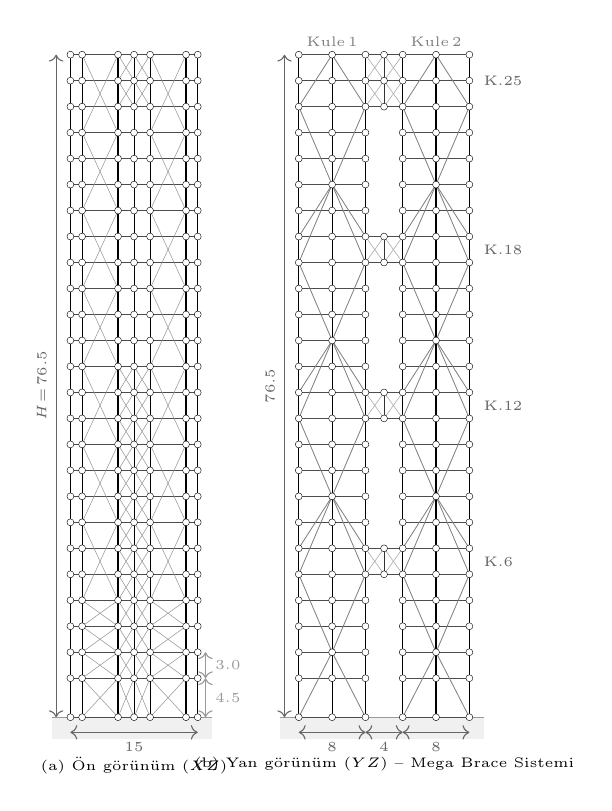
\begin{tikzpicture}[font=\scriptsize]
\pgfmathsetmacro{\s}{0.055}
% ===== (a) ÖN GÖRÜNÜM (XZ düzlemi) =====
\begin{scope}[xscale=\s, yscale=\s]
% Zemin
\fill[black!6] (-4,-5) rectangle (33,0);
\draw[black!40] (-4,0) -- (33,0);
% --- Kolonlar (siyah) ---
\foreach \x in {0.3,3,11.3,15,18.7,27,29.7} {
  \draw[black, line width=0.4pt] (\x,0) -- (\x,153);
}
% --- Kirişler beam_x: her kat (koyu gri) ---
\draw[black!70, line width=0.2pt] (0.3,0) -- (29.7,0);
\draw[black!70, line width=0.2pt] (0.3,9) -- (29.7,9);
\foreach \f in {2,...,25} {
  \pgfmathsetmacro{\z}{9+(\f-1)*6}
  \draw[black!70, line width=0.2pt] (0.3,\z) -- (29.7,\z);
}
% --- Çapraz XZ: iç 3.7cm açıklıklar, X-cross kat 0--12 + son 2 kat (açık gri) ---
\foreach \za/\zb in {0/9,9/15,15/21,21/27,27/33,33/39,39/45,45/51,51/57,57/63,63/69,69/75,75/81,141/147,147/153} {
  \foreach \xa/\xb in {11.3/15,15/18.7} {
    \draw[black!40, line width=0.2pt] (\xa,\za)--(\xb,\zb);
    \draw[black!40, line width=0.2pt] (\xb,\za)--(\xa,\zb);
  }
}
% --- Çapraz XZ: 8cm açıklıklar (3-11, 19-27), ilk 4 kat tek, sonra 3'er katlık (açık gri) ---
\foreach \za/\zb in {0/9,9/15,15/21,21/27,27/45,45/63,63/81,81/99,99/117,117/135,135/153} {
  \foreach \xa/\xb in {3/11.3,18.7/27} {
    \draw[black!40, line width=0.2pt] (\xa,\za)--(\xb,\zb);
    \draw[black!40, line width=0.2pt] (\xb,\za)--(\xa,\zb);
  }
}
% --- Düğüm noktaları (beyaz dolu daire) ---
\foreach \x in {0.3,3,11.3,15,18.7,27,29.7} {
  % Zemin kat
  \fill[white] (\x,0) circle (0.8); \draw[black, line width=0.15pt] (\x,0) circle (0.8);
  % 1. kat (z=9)
  \fill[white] (\x,9) circle (0.8); \draw[black, line width=0.15pt] (\x,9) circle (0.8);
  % Üst katlar
  \foreach \f in {2,...,25} {
    \pgfmathsetmacro{\z}{9+(\f-1)*6}
    \fill[white] (\x,\z) circle (0.8); \draw[black, line width=0.15pt] (\x,\z) circle (0.8);
  }
}
% --- Ölçüler ---
\draw[<->,thin,black!60] (-3,0) -- node[left,font=\tiny,rotate=90,anchor=south]{$H\!=\!76.5$} (-3,153);
\draw[<->,thin,black!60] (0.3,-3.5) -- node[below,font=\tiny]{$15$} (29.7,-3.5);
\draw[<->,thin,black!40] (31.5,0) -- node[right,font=\tiny]{$4.5$} (31.5,9);
\draw[<->,thin,black!40] (31.5,9) -- node[right,font=\tiny]{$3.0$} (31.5,15);
% Alt başlık
\node[font=\tiny,anchor=north] at (15,-7) {(a) Ön görünüm ($XZ$)};
\end{scope}
% ===== (b) YAN GÖRÜNÜM (YZ düzlemi) =====
\begin{scope}[shift={(2.9,0)}, xscale=\s, yscale=\s]

% --- Arka Plan ve Zemin ---
\fill[black!6] (-4,-5) rectangle (43,0);
\draw[black!40] (-4,0) -- (43,0);

% ==========================================
% 1. KOLONLAR VE KİRİŞLER (Sabit Yapı)
% ==========================================

% --- Kolonlar Kule 1 (Sol) ---
\foreach \y in {0.3,8,15.7} { \draw[black, line width=0.4pt] (\y,0) -- (\y,153); }
% --- Kolonlar Kule 2 (Sağ) ---
\foreach \y in {24.3,32,39.7} { \draw[black, line width=0.4pt] (\y,0) -- (\y,153); }

% --- Kirişler (Kat Döşemeleri) ---
% Zemin ve 1. Kat
\foreach \towerL/\towerR in {0.3/15.7, 24.3/39.7} {
    \draw[black!70, line width=0.2pt] (\towerL,0)--(\towerR,0);
    \draw[black!70, line width=0.2pt] (\towerL,9)--(\towerR,9);
}
% Üst Katlar (2. kattan 25. kata kadar)
\foreach \f in {2,...,25} {
    \pgfmathsetmacro{\z}{9+(\f-1)*6}
    \draw[black!70, line width=0.2pt] (0.3,\z)--(15.7,\z);   % Kule 1
    \draw[black!70, line width=0.2pt] (24.3,\z)--(39.7,\z); % Kule 2
}

% ==========================================
% 2. YENİ ÇAPRAZ SİSTEMİ (Mega Brace)
% ==========================================

% --- (A) ZEMİN BLOĞU (0m -> 33m) ---
% Z=0 (Zemin) -> Z=15 (2. Kat, Orta) -> Z=33 (Köprü 1 Altı)
\foreach \midX/\leftX/\rightX in {8/0.3/15.7, 32/24.3/39.7} {
    % Alt Parça: Zeminden Ortaya (0 -> 15)
    \draw[black!50, line width=0.3pt] (\leftX,0) -- (\midX,15);
    \draw[black!50, line width=0.3pt] (\rightX,0) -- (\midX,15);
    % Üst Parça: Ortadan Köprü Altına (15 -> 33)
    \draw[black!50, line width=0.3pt] (\midX,15) -- (\leftX,33);
    \draw[black!50, line width=0.3pt] (\midX,15) -- (\rightX,33);
}

% --- (B) ARA BLOKLAR (Mega Brace: Köprü Altı -> Köprü Altı) ---
% 1. Modül: Köprü 1 Altı (33) -> Köprü 2 Altı (69). Merkez Z=51. Köprü 1 Üstü=39.
% 2. Modül: Köprü 2 Altı (69) -> Köprü 3 Altı (105). Merkez Z=87. Köprü 2 Üstü=75.
% 3. Modül: Köprü 3 Altı (105) -> Köprü 4 Altı (141). Merkez Z=123. Köprü 3 Üstü=111.

\foreach \zBot/\zTop/\zMid/\zBridgeTop in {33/69/51/39, 69/105/87/75, 105/141/123/111} {
    \foreach \midX/\leftX/\rightX in {8/0.3/15.7, 32/24.3/39.7} {
        % 1. Ana Elmas: Köprü Altından (zBot) Mega Merkeze (zMid)
        \draw[black!50, line width=0.3pt] (\leftX, \zBot) -- (\midX, \zMid);
        \draw[black!50, line width=0.3pt] (\rightX, \zBot) -- (\midX, \zMid);
        
        % 2. Ana Elmas: Mega Merkezden (zMid) Bir Sonraki Köprü Altına (zTop)
        \draw[black!50, line width=0.3pt] (\midX, \zMid) -- (\leftX, \zTop);
        \draw[black!50, line width=0.3pt] (\midX, \zMid) -- (\rightX, \zTop);
        
        % 3. Ek Bağlantı: Köprü Üstü -> Mega Brace Merkezi
        \draw[black!50, line width=0.3pt] (\leftX, \zBridgeTop) -- (\midX, \zMid);
        \draw[black!50, line width=0.3pt] (\rightX, \zBridgeTop) -- (\midX, \zMid);
    }
}

% --- (C) EN ÜST KAT (141m -> 153m) ---
\foreach \midX/\leftX/\rightX in {8/0.3/15.7, 32/24.3/39.7} {
    \draw[black!50, line width=0.3pt] (\leftX, 141) -- (\midX, 153);
    \draw[black!50, line width=0.3pt] (\rightX, 141) -- (\midX, 153);
}

% ==========================================
% 3. KÖPRÜLER (Yatay Bağlantılar)
% ==========================================
\foreach \za/\zb in {33/39, 69/75, 105/111} {
    % Kolon
    \draw[black!80, line width=0.4pt] (20,\za)--(20,\zb);
    % Kirişler
    \draw[black!70, line width=0.3pt] (15.7,\za)--(24.3,\za);
    \draw[black!70, line width=0.3pt] (15.7,\zb)--(24.3,\zb);
    % Çapraz kafes
    \draw[black!35, line width=0.2pt] (15.7,\za)--(20,\zb);
    \draw[black!35, line width=0.2pt] (20,\za)--(15.7,\zb);
    \draw[black!35, line width=0.2pt] (20,\za)--(24.3,\zb);
    \draw[black!35, line width=0.2pt] (24.3,\za)--(20,\zb);
}

% --- En Üst Köprü (Çift katmanlı) ---
\draw[black!80, line width=0.4pt] (20,141)--(20,153);
\draw[black!70, line width=0.3pt] (15.7,141)--(24.3,141);
\draw[black!70, line width=0.3pt] (15.7,147)--(24.3,147);
\draw[black!70, line width=0.3pt] (15.7,153)--(24.3,153);
% Kafes
\draw[black!35, line width=0.2pt] (15.7,141)--(20,147);
\draw[black!35, line width=0.2pt] (20,141)--(15.7,147);
\draw[black!35, line width=0.2pt] (20,141)--(24.3,147);
\draw[black!35, line width=0.2pt] (24.3,141)--(20,147);
\draw[black!35, line width=0.2pt] (15.7,147)--(20,153);
\draw[black!35, line width=0.2pt] (20,147)--(15.7,153);
\draw[black!35, line width=0.2pt] (20,147)--(24.3,153);
\draw[black!35, line width=0.2pt] (24.3,147)--(20,153);

% ==========================================
% 4. DÜĞÜM NOKTALARI
% ==========================================
\foreach \y in {0.3,8,15.7, 24.3,32,39.7} {
    % Zemin
    \fill[white] (\y,0) circle (0.8); \draw[black, line width=0.15pt] (\y,0) circle (0.8);
    % 1. Kat
    \fill[white] (\y,9) circle (0.8); \draw[black, line width=0.15pt] (\y,9) circle (0.8);
    % Diğer Katlar
    \foreach \f in {2,...,25} {
        \pgfmathsetmacro{\z}{9+(\f-1)*6}
        \fill[white] (\y,\z) circle (0.8); \draw[black, line width=0.15pt] (\y,\z) circle (0.8);
    }
}
% Köprü Düğüm Noktaları (Orta)
\foreach \za in {33,39,69,75,105,111,141,147,153} {
    \fill[white] (20,\za) circle (0.8); \draw[black, line width=0.15pt] (20,\za) circle (0.8);
}

% ==========================================
% 5. ETİKETLER VE ÖLÇÜLER
% ==========================================
\node[font=\tiny,black!50] at (8,156) {Kule\,1};
\node[font=\tiny,black!50] at (32,156) {Kule\,2};

\node[font=\tiny,black!60,anchor=west] at (40.8,36) {K.6};
\node[font=\tiny,black!60,anchor=west] at (40.8,72) {K.12};
\node[font=\tiny,black!60,anchor=west] at (40.8,108) {K.18};
\node[font=\tiny,black!60,anchor=west] at (40.8,147) {K.25};

\draw[<->,thin,black!60] (0.3,-3.5) -- node[below,font=\tiny]{$8$} (15.7,-3.5);
\draw[<->,thin,black!60] (15.7,-3.5) -- node[below,font=\tiny]{$4$} (24.3,-3.5);
\draw[<->,thin,black!60] (24.3,-3.5) -- node[below,font=\tiny]{$8$} (39.7,-3.5);
\draw[<->,thin,black!60] (-3,0) -- node[left,font=\tiny,rotate=90,anchor=south]{$76.5$} (-3,153);

\node[font=\tiny,anchor=north] at (20,-7) {(b) Yan görünüm ($YZ$) -- Mega Brace Sistemi};

\end{scope}
\end{tikzpicture}%
}
\caption{V10 modelinin yapısal sistemi: (a)~ön görünüm ($XZ$)---iç açıklıklarda X-çapraz (0--12.~kat), dış açıklıklarda 3~katlık zikzak; (b)~yan görünüm ($YZ$)---mega brace çapraz sistemi ve köprü kafes bağlantıları. Siyah: kolon, koyu gri: kiriş/köprü, açık gri: çapraz. Beyaz daireler: düğüm noktaları. Ölçüler metre cinsindendir.}
\label{fig:sistem}
\end{figure}


\newpage

% --- 4. ÇİZİMLER ---
\section{ÇİZİMLER}
Binanın her bir farklı katına ait plan ve iki ana doğrultudaki kesit çizimleri verilecektir.
\begin{itemize}
    \item Çizimler ayrıca "dwg" formatında ek olarak sunulacaktır.
\end{itemize}

\newpage

% ################### SORULAR VE CEVAPLAR ###################

% ==============================================================================
% SORU 1
% ==============================================================================
\section{SORULAR}
\subsection{Soru \RN{1}}

\textbf{Soru:} Yapı taşıyıcı sistemini belirlerken nelere dikkat ettiğinizi depreme dayanıklı bina tasarım ilkeleri çerçevesinde (taşıyıcı elemanların geometrisi ve yerleşimi, yeterli dayanım, rijitlik ve sünekliğin sağlanması gibi) açıklayınız.

\textbf{Cevap:} Taşıyıcı sistem seçiminde beş temel ilkeye dikkat edilmiştir: (1)~simetri ve düzenlilik, (2)~yeterli rijitlik, (3)~sürekli yük aktarımı, (4)~süneklik, (5)~hafiflik. TBDY 2018 ve uluslararası tasarım esasları çerçevesinde bu ilkeler aşağıda açıklanmıştır~\cite{tbdy2018, nehrp2009}.

\subsubsection{İkiz Kule ve Köprü Sistemi \& Simetri ve Düzenlilik}

Yüksek katlı yapı konfigürasyonu olarak iki ayrı kule ve bunları birbirine bağlayan köprü elemanlarından oluşan bir sistem tasarlanmıştır. Her kule 26 kattan oluşmakta olup $7 \times 3$ kolon gridi üzerine inşa edilmiştir. Literatürdeki çalışmalar, köprü bağlantılarının yapı yüksekliğinin $1/4$, $1/2$ ve $3/4$ seviyelerine yerleştirilmesinin sismik performansı optimize ettiğini göstermektedir~\cite{patoliya2023}. Bu doğrultuda köprüler yaklaşık olarak 6., 12., 18. ve 25. katlara konumlandırılmıştır. Bu konfigürasyon, yatay yükler altında kulelerin birlikte çalışmasını sağlamakta ve tek bir yüksek kuleye kıyasla daha dengeli yük dağılımı sunmaktadır. Yapının planda ve düşeyde düzenli olması, burulma düzensizliğini önlemek açısından temel gerekliliktir. İkiz kule sistemi her iki ana eksende ($X$, $Y$) simetrik olarak tasarlanmış; kütle merkezi ile rijitlik merkezi arasındaki eksantrisite en aza indirilmiştir. A1a burulma düzensizliği katsayısı zemin katta $\eta_{bi} = 1.69$ olup $2{,}0$'nin altındadır; üst katlarda $\eta_{bi} < 1.2$ değerleri elde edilmiştir~\cite{teblig2024}.

\subsubsection{Yeterli Yanal Rijitlik \& Sürekli Yük Aktarımı ve Süneklik}

Deprem yüklerinin güvenle temele aktarılması için yapının yatay kuvvetlere karşı yeterli rijitliğe sahip olması gerekmektedir. Çerçeve-çapraz hibrit sistem tercih edilerek, moment taşıyan çerçevelerin sünekliği ile çapraz elemanların rijitliği bir arada kullanılmıştır. Çapraz elemanlar $XZ$ ve $YZ$ düzlemlerinde stratejik noktalara yerleştirilmiş; köprü bağlantısı ise iki kule arasında yük paylaşımını sağlayarak global sistem rijitliğini artırmıştır. Deprem yüklerinin kesintisiz olarak temele iletilmesi için düşey taşıyıcı elemanlar tüm katlarda aynı konumda devam etmektedir. Kolon-kiriş düğüm noktaları rijit bağlantılı, çapraz elemanlar mafsallı modellenmiştir. Güçlü kolon--zayıf kiriş tasarım prensibi uygulanarak plastik mafsalların kiriş uçlarında oluşması hedeflenmiştir. CQC yöntemiyle hesaplanan göreli kat ötelemesi $\delta/h = 0.00117 < 0.008$'dir~\cite{tbdy2018}.

\subsubsection{Hafiflik ve Malzeme}

Deprem kuvvetleri yapı kütlesi ile doğru orantılı olduğundan, taşıyıcı sistemin mümkün olduğunca hafif tutulması esastır. Balsa ahşap malzeme ($E = 3.5$~GPa) kullanılarak yapısal analizler \textsc{OpenSees}\textsuperscript{\textregistered} yazılımı ile gerçekleştirilmiş~\cite{opensees}, ağırlık minimizasyonu ve rijitlik maksimizasyonu hedefleriyle iteratif optimizasyon yapılmıştır. \href{https://github.com/adzetto/DASK_26__DESIGN_AND_ANALYSIS}{\textcolor{blue}{Github deposunda}} tüm analiz ve optimizasyon kodları mevcuttur~\cite{github_repo}.

Sonuç olarak, sahaya özgü deprem tehlikesi parametreleri ($S_{DS} = 1.008$~g, $S_{D1} = 0.514$~g, zemin sınıfı ZD) dikkate alınarak~\cite{afad2024}, TBDY 2018 gerekliliklerini karşılayan simetrik, yeterli yanal rijitliğe ve sünekliğe sahip, hafif bir çerçeve--çapraz hibrit ikiz kule--köprü taşıyıcı sistemi tasarlanmıştır.

\newpage

% ==============================================================================
% SORU 2 (Placeholder)
% ==============================================================================
\subsection{Soru \RN{2}}

\textbf{Soru:} Binanızın doğal titreşim periyodu ile deprem yer hareketi tepki spektrumu arasındaki ilişkiyi açıklayınız.

\textbf{Cevap:} Yapının ilk üç doğal titreşim periyodu ($T_1=0.115$~s, $T_2=0.079$~s, $T_3=0.054$~s) değerlendirildiğinde, $T_1$ TBDY~2018 DD-2 tasarım spektrumunun sabit ivme (plato) bölgesine ($T_A=0.102$~s $< T_1 <$ $T_B=0.510$~s) düşmekte; $T_2$ ve $T_3$ ise artan bölgede ($T < T_A$) yer almaktadır. Birinci mod tam plato ivmesini ($S_{ae}=1.008$~g) alırken, $T_2$ için $S_{ae}=0.872$~g, $T_3$ için $S_{ae}=0.723$~g elde edilmektedir. Periyotların ZD zemin hakim periyodundan ($T_g\approx0.4$--$0.7$~s) belirgin şekilde kısa olması rezonans riskini ortadan kaldırmaktadır.

İstanbul Finans Merkezi ($41.002136^\circ$, $29.106832^\circ$) için AFAD~\cite{afad2024} DD-2 verileri: $S_S = 0.877$, $S_1 = 0.243$, zemin sınıfı ZD. Yerel zemin etki katsayıları $F_S = 1.149$, $F_1 = 2.114$ ile tasarım parametreleri:
%
\begin{equation}
S_{DS} = 0.877 \times 1.149 = 1.008\text{~g}, \quad S_{D1} = 0.243 \times 2.114 = 0.514\text{~g}.
\end{equation}
%
Köşe periyotları $T_A = 0.2 \cdot S_{D1}/S_{DS} = 0.102$~s, $T_B = S_{D1}/S_{DS} = 0.510$~s olarak hesaplanmıştır~\cite{tbdy2018}.

\textsc{OpenSees}\textsuperscript{\textregistered}~\cite{opensees} ile 1108 düğüm, 2794~elemanlı V10 modeli \texttt{elasticBeamColumn} elemanları ve toplu kütle (\textit{lumped mass}) formülasyonu ile oluşturulmuştur. Özdeğer problemi $\mathbf{K}\boldsymbol{\phi}_n = \omega_n^2 \mathbf{M}\boldsymbol{\phi}_n$ ARPACK kütüphanesi ile Lanczos iterasyonu (\texttt{-genBandArpack}) kullanılarak çözülmüş; ilk 12~mod için periyotlar $T_n = 2\pi/\omega_n$ ile elde edilmiştir. Modal periyotlar: $T_1 = 0.115$~s (Y sallanım, \%72.3), $T_2 = 0.079$~s (X sallanım, \%68.3), $T_3 = 0.054$~s (burulma). Birinci mod $T_A < T_1 < T_B$ aralığında plato bölgesinde olup $S_{ae} = S_{DS} = 1.008$~g almaktadır; $T_2$ ve $T_3$ artan bölgede olup $S_{ae}(T_2) = 0.872$~g, $S_{ae}(T_3) = 0.723$~g değerlerini almaktadır. Dördüncü mod ($T_4 = 0.039$~s) daha derin artan bölgede: $S_{ae}(T_4) = (0.4 + 0.6 \cdot 0.039/0.102) \cdot 1.008 = 0.635$~g. Modal katkılar CQC yöntemiyle birleştirilmiş olup korelasyon katsayısı $\rho_{ij} = 8\xi^2(1+\beta_{ij})\beta_{ij}^{3/2}/[(1-\beta_{ij}^2)^2 + 4\xi^2\beta_{ij}(1+\beta_{ij})^2]$ ($\beta_{ij} = \omega_i/\omega_j$, $\xi = 0.05$) ile hesaplanmıştır. Elastik taban kesme kuvveti $V_t = 160$~N olup TBDY~2018 gerekliliklerini sağlamaktadır. Yapı periyodunun ZD zemin hakim periyodundan ($T_g \approx 0.4$--$0.7$~s) kısa olması rezonans riskini azaltmaktadır. Spektrum-periyot ilişkisi Şekil~\ref{fig:spectrum}'de gösterilmektedir.

% ==============================================================================
% ŞEKİL: AFAD Tasarım Spektrumları ve Modal Analiz
% ==============================================================================
\begin{figure}[H]
\centering
\resizebox{0.65\textwidth}{!}{%
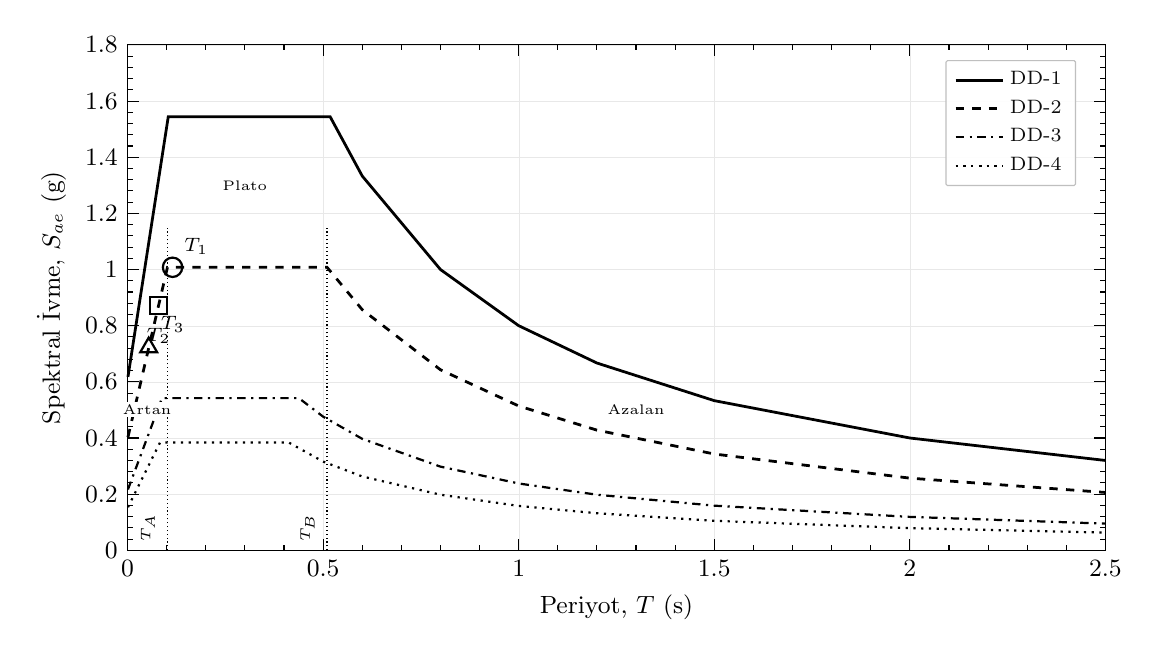
\begin{tikzpicture}
\begin{axis}[
    sciencestyle,
    width=14cm,
    height=8cm,
    xlabel={Periyot, $T$ (s)},
    ylabel={Spektral İvme, $S_{ae}$ (g)},
    xmin=0, xmax=2.5,
    ymin=0, ymax=1.8,
    xtick={0,0.5,1.0,1.5,2.0,2.5},
    ytick={0,0.2,0.4,0.6,0.8,1.0,1.2,1.4,1.6,1.8},
    minor tick num=4,
    legend pos=north east,
    clip=false,
]

% DD-1 Spektrumu
\addplot[black, solid, line width=1.0pt] coordinates {
    (0.001, 0.6176) (0.104, 1.544) (0.518, 1.544) (0.6, 1.333) (0.8, 1.0) (1.0, 0.8) (1.2, 0.667) (1.5, 0.533) (2.0, 0.4) (2.5, 0.32)
};

% DD-2 Spektrumu
\addplot[black, dashed, line width=1.0pt] coordinates {
    (0.001, 0.4032) (0.102, 1.008) (0.510, 1.008) (0.6, 0.857) (0.8, 0.643) (1.0, 0.514) (1.2, 0.428) (1.5, 0.343) (2.0, 0.257) (2.5, 0.206)
};

% DD-3 Spektrumu
\addplot[black, dashdotted, line width=0.8pt] coordinates {
    (0.001, 0.2168) (0.088, 0.542) (0.438, 0.542) (0.5, 0.476) (0.6, 0.397) (0.8, 0.298) (1.0, 0.238) (1.2, 0.198) (1.5, 0.159) (2.0, 0.119) (2.5, 0.095)
};

% DD-4 Spektrumu
\addplot[black, dotted, line width=0.8pt] coordinates {
    (0.001, 0.1536) (0.083, 0.384) (0.412, 0.384) (0.5, 0.316) (0.6, 0.263) (0.8, 0.198) (1.0, 0.158) (1.2, 0.132) (1.5, 0.105) (2.0, 0.079) (2.5, 0.063)
};

% Modal Analiz - Mod 1 (plato)
\addplot[only marks, mark=o, mark size=3.5pt, fill=white, draw=black, line width=0.8pt] coordinates {(0.115, 1.008)};
\node[anchor=south west, font=\scriptsize] at (axis cs:0.120, 1.020) {$T_1$};

% Mod 2 (artan bölge)
\addplot[only marks, mark=square, mark size=3pt, fill=white, draw=black, line width=0.8pt] coordinates {(0.079, 0.872)};
\node[anchor=south, font=\scriptsize] at (axis cs:0.079, 0.700) {$T_2$};

% Mod 3 (artan bölge)
\addplot[only marks, mark=triangle, mark size=3.5pt, fill=white, draw=black, line width=0.8pt] coordinates {(0.054, 0.723)};
\node[anchor=south west, font=\scriptsize] at (axis cs:0.060, 0.740) {$T_3$};

% Köşe periyotları
\addplot[black, thin, densely dotted] coordinates {(0.102, 0) (0.102, 1.15)};
\node[anchor=south, font=\tiny, rotate=90] at (axis cs:0.095, 0.08) {$T_A$};

\addplot[black, thin, densely dotted] coordinates {(0.510, 0) (0.510, 1.15)};
\node[anchor=south, font=\tiny, rotate=90] at (axis cs:0.503, 0.08) {$T_B$};

% Bölge etiketleri
\node[anchor=center, font=\tiny, fill=white, inner sep=1pt] at (axis cs:0.05, 0.50) {Artan};
\node[anchor=center, font=\tiny, fill=white, inner sep=1pt] at (axis cs:0.30, 1.30) {Plato};
\node[anchor=center, font=\tiny, fill=white, inner sep=1pt] at (axis cs:1.3, 0.5) {Azalan};

\legend{DD-1, DD-2, DD-3, DD-4}

\end{axis}
\end{tikzpicture}%
}
\caption{AFAD DD-1/2/3/4 yatay elastik tasarım spektrumları ve \textsc{OpenSees} modal analiz sonuçları (İFM, ZD). Beyaz işaretçiler V10 modelinin ilk üç modunu göstermektedir ($T_1 = 0.115$~s plato, $T_2 = 0.079$~s artan, $T_3 = 0.054$~s artan).}
\label{fig:spectrum}
\end{figure}



\newpage

% ==============================================================================
% SORU 3 (Placeholder)
% ==============================================================================
\subsection{Soru \RN{3}}

\textbf{Soru:} Yapıdaki düşey taşıyıcıların yerleşiminin belirlenmesinde dikkat edilen hususlar nelerdir?

\textbf{Cevap:} Düşey taşıyıcı yerleşiminde üç temel hedef gözetilmiştir: (i)~düşey yüklerin ($Z$) sürekli ve kesintisiz temele aktarımı, (ii)~yatay kuvvetlere ($X$, $Y$) karşı yeterli yanal rijitliğin temini, (iii)~burulma düzensizliğinin kontrolü~\cite{tbdy2018}.

\textit{Kolon Grid Konfigürasyonu:} Her kule için $7 \times 3$ ortogonal kolon gridi uygulanmıştır. $X$ ekseninde değişken açıklık düzeni benimsenmiş olup köşe açıklıkları ($L = 2{,}7$~cm) kısa tutularak moment çerçevesi rijitliği artırılmış, iç açıklıklarda ($3{,}7$~cm) perde duvarı benzeri rijitlik konsantrasyonu sağlanmıştır. $Y$ ekseninde eşit iki açıklık ($L_y = 7{,}7$~cm) ile simetrik dağılım elde edilmiş; merkez kolonlar köprü bağlantı hattını güçlendirmektedir. Bu konfigürasyon rijitlik merkezi ile kütle merkezi arasındaki mesafeyi sıfıra indirerek burulma talebini azaltmaktadır~\cite{nehrp2009}.

\textit{Yanal Yük Taşıyıcı Sistem:} Moment çerçevesi tek başına hedef yanal rijitliği karşılayamadığından, $XZ$ ve $YZ$ düzlemlerinde çapraz elemanlarla desteklenmiş hibrit sistem tercih edilmiştir. Çapraz elemanlar köşe ve merkez açıklıklara yerleştirilmiş; tüm katlarda kesintisiz devam ettirilerek yük akışı sürekliliği tesis edilmiştir~\cite{tbdy2018}.

\textit{Köprü Bağlantı Seviyeleri:} Köprüler yapı yüksekliğinin $H/4$, $H/2$, $3H/4$ ve tepe kotlarına konumlandırılmıştır. Bu dağılım, ikiz kule sistemlerinde mod şekillerini dengeleyerek taban kesme kuvvetini minimize etmektedir~\cite{patoliya2023}. Köprü genişliği merkez kolon hattı ($x = 11.3$--$18.7$~cm, genişlik $7{,}4$~cm) ile sınırlandırılmış; böylece kulelerin bağımsız titreşim karakteristiği korunarak kontrollü yük paylaşımı sağlanmıştır. Uygulanan çift simetri sayesinde kütle-rijitlik eksantrisitesi $e_x/L_x = 0{,}000$, $e_y/L_y = 0{,}000$ olarak elde edilmiştir~\cite{tbdy2018}. Zemin katta A1a burulma düzensizliği katsayısı $\eta_{bi} = 1{,}69 < 2{,}0$ olup bu değer alt katlardaki asimetrik çapraz rijitliğinden kaynaklanmaktadır; 5.~kattan itibaren $\eta_{bi} < 1{,}2$ değerleri elde edilmiştir~\cite{teblig2024}. Kolon yerleşimi Şekil~\ref{fig:plan}'de sunulmaktadır.

% ==============================================================================
% ŞEKİL: Kolon Yerleşimi ve Köprü Bağlantısı (Kesit + Plan)
% ==============================================================================
\begin{figure}[H]
\centering
\resizebox{0.95\textwidth}{!}{%
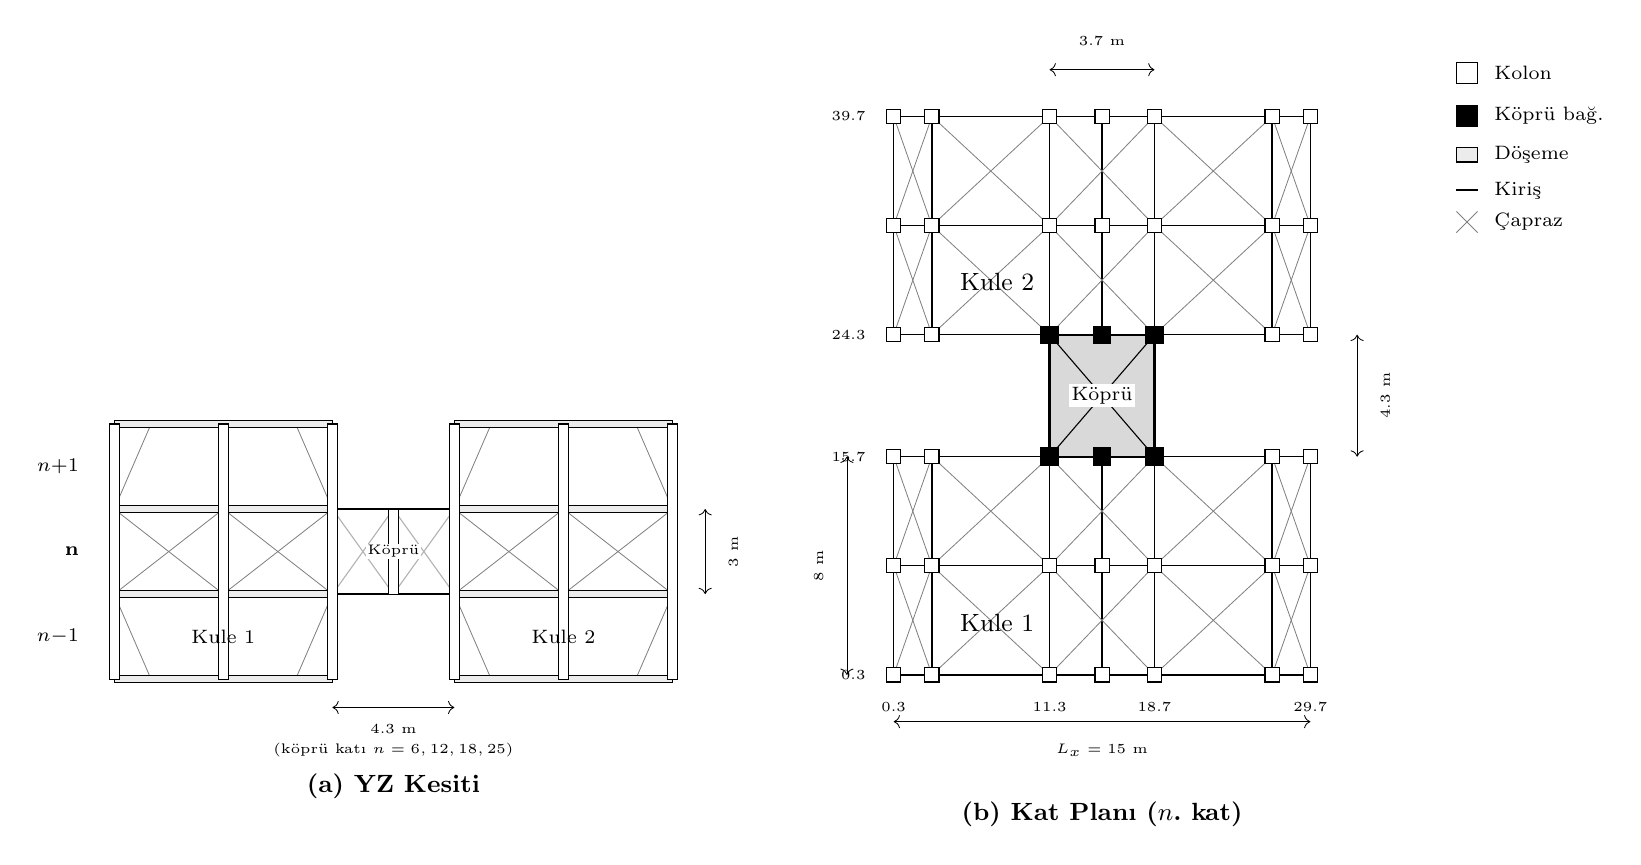
\begin{tikzpicture}[scale=0.18]

% ============== SOL: KESİT GÖRÜNÜMÜ (YZ düzlemi) ==============
\begin{scope}[shift={(0,0)}]
\def\kh{6}
% 4 döşeme seviyesi: z=0, 6, 12, 18  (sürekli, boşluksuz)
% n-1: z=0→6  |  n (köprü): z=6→12  |  n+1: z=12→18

% --- 1. Çaprazlar (arka plan) ---
% n-1 katı kule çaprazları (Alttan Gelen - Köşeye Gidiyor)
% Global: Floor 5 (n-1). Node at Floor 6 (n).
% Interpolation: Bottom(n-1) is 2/3 from Center to Corner. Top(n-1) is Corner.
\draw[line width=0.3pt, gray] (2.9,0) -- (0.3,\kh);
\draw[line width=0.3pt, gray] (13.1,0) -- (15.7,\kh);
\draw[line width=0.3pt, gray] (26.9,0) -- (24.3,\kh);
\draw[line width=0.3pt, gray] (37.1,0) -- (39.7,\kh);

% n katı kule çaprazları (Köprü Katı - Güçlü Düğüm - Kule İçi X)
% Her iki açıklıkta küçük X
\draw[line width=0.3pt, gray] (0.3,\kh) -- (8.0,2*\kh); \draw[line width=0.3pt, gray] (8.0,\kh) -- (0.3,2*\kh);
\draw[line width=0.3pt, gray] (8.0,\kh) -- (15.7,2*\kh); \draw[line width=0.3pt, gray] (15.7,\kh) -- (8.0,2*\kh);
\draw[line width=0.3pt, gray] (24.3,\kh) -- (32.0,2*\kh); \draw[line width=0.3pt, gray] (32.0,\kh) -- (24.3,2*\kh);
\draw[line width=0.3pt, gray] (32.0,\kh) -- (39.7,2*\kh); \draw[line width=0.3pt, gray] (39.7,\kh) -- (32.0,2*\kh);

% n katı köprü çaprazları (orta kolon ile ikiye ayrılmış X-çapraz)
\draw[line width=0.4pt, gray!60] (15.7,\kh) -- (20.0,2*\kh);
\draw[line width=0.4pt, gray!60] (20.0,\kh) -- (15.7,2*\kh);
\draw[line width=0.4pt, gray!60] (20.0,\kh) -- (24.3,2*\kh);
\draw[line width=0.4pt, gray!60] (24.3,\kh) -- (20.0,2*\kh);

% n+1 katı kule çaprazları (Üste Giden - Merkezden Gidiyor)
% Global: Floor 7 (n+1). Node at Floor 6 (n).
% Interpolation: Bottom(n+1) is Corner. Top(n+1) is 1/3 to Center.
\draw[line width=0.3pt, gray] (0.3,2*\kh) -- (2.9,3*\kh);
\draw[line width=0.3pt, gray] (15.7,2*\kh) -- (13.1,3*\kh);
\draw[line width=0.3pt, gray] (24.3,2*\kh) -- (26.9,3*\kh);
\draw[line width=0.3pt, gray] (39.7,2*\kh) -- (37.1,3*\kh);

% --- 2. Döşemeler (kat seviyelerinde yatay plaklar) ---
% z=0: alt döşeme (yalnız kuleler)
\draw[fill=gray!15, draw=black, line width=0.5pt] (0.3,-0.25) rectangle (15.7,0.25);
\draw[fill=gray!15, draw=black, line width=0.5pt] (24.3,-0.25) rectangle (39.7,0.25);
% z=6: n-1/n ara döşeme + köprü kirişi
\draw[fill=gray!15, draw=black, line width=0.5pt] (0.3,\kh-0.25) rectangle (15.7,\kh+0.25);
\draw[line width=0.6pt] (15.7,\kh) -- (24.3,\kh);
\draw[fill=gray!15, draw=black, line width=0.5pt] (24.3,\kh-0.25) rectangle (39.7,\kh+0.25);
% z=12: n/n+1 ara döşeme + köprü kirişi
\draw[fill=gray!15, draw=black, line width=0.5pt] (0.3,2*\kh-0.25) rectangle (15.7,2*\kh+0.25);
\draw[line width=0.6pt] (15.7,2*\kh) -- (24.3,2*\kh);
\draw[fill=gray!15, draw=black, line width=0.5pt] (24.3,2*\kh-0.25) rectangle (39.7,2*\kh+0.25);
% z=18: üst döşeme (yalnız kuleler)
\draw[fill=gray!15, draw=black, line width=0.5pt] (0.3,3*\kh-0.25) rectangle (15.7,3*\kh+0.25);
\draw[fill=gray!15, draw=black, line width=0.5pt] (24.3,3*\kh-0.25) rectangle (39.7,3*\kh+0.25);

% --- 3. Kolonlar (beyaz dolgu, sürekli tüm katlar boyunca) ---
\foreach \y in {0.3,8.0,15.7,24.3,32.0,39.7} {
    \draw[fill=white, draw=black, line width=0.4pt] (\y-0.35,0) rectangle (\y+0.35,3*\kh);
}
% Köprü orta kolonu (yalnız n katı boyunca)
\draw[fill=white, draw=black, line width=0.4pt] (20-0.35,\kh) rectangle (20+0.35,2*\kh);

% --- 4. Etiketler ---
\node[font=\scriptsize, anchor=east] at (-1.5,\kh/2) {$n{-}1$};
\node[font=\scriptsize, anchor=east] at (-1.5,1.5*\kh) {\textbf{n}};
\node[font=\scriptsize, anchor=east] at (-1.5,2.5*\kh) {$n{+}1$};
\node[font=\scriptsize] at (8,\kh/2) {Kule 1};
\node[font=\scriptsize] at (32,\kh/2) {Kule 2};
\node[font=\tiny, fill=white, inner sep=0.5pt] at (20,1.5*\kh) {Köprü};

% --- 5. Boyutlar ---
\draw[<->, line width=0.3pt] (15.7,-2) -- (24.3,-2);
\node[font=\tiny] at (20,-3.5) {4.3 m};
\draw[<->, line width=0.3pt] (42,\kh) -- (42,2*\kh);
\node[font=\tiny, rotate=90] at (44,1.5*\kh) {3 m};

\node[font=\small, anchor=north] at (20,-6) {\textbf{(a) YZ Kesiti}};
\node[font=\tiny] at (20,-5) {(köprü katı $n = 6, 12, 18, 25$)};
\end{scope}

% ============== SAĞ: PLAN GÖRÜNÜMÜ (n. kat) ==============
\begin{scope}[shift={(55,0)}]

% Kirişler X yönü (Kule 1)
\foreach \y in {0.3,8.0,15.7} {
    \draw[line width=0.5pt] (0.3,\y) -- (29.7,\y);
}
% Kirişler X yönü (Kule 2)
\foreach \y in {24.3,32.0,39.7} {
    \draw[line width=0.5pt] (0.3,\y) -- (29.7,\y);
}
% Kirişler Y yönü (Kule 1)
\foreach \x in {0.3,3.0,11.3,15.0,18.7,27.0,29.7} {
    \draw[line width=0.5pt] (\x,0.3) -- (\x,15.7);
}
% Kirişler Y yönü (Kule 2)
\foreach \x in {0.3,3.0,11.3,15.0,18.7,27.0,29.7} {
    \draw[line width=0.5pt] (\x,24.3) -- (\x,39.7);
}

% Döşeme çaprazları (Kule 1) - tüm paneller
% Köşe sol
\draw[line width=0.3pt, gray] (0.3,0.3) -- (3.0,8.0);
\draw[line width=0.3pt, gray] (3.0,0.3) -- (0.3,8.0);
\draw[line width=0.3pt, gray] (27.0,0.3) -- (29.7,8.0);
\draw[line width=0.3pt, gray] (29.7,0.3) -- (27.0,8.0);
\draw[line width=0.3pt, gray] (0.3,8.0) -- (3.0,15.7);
\draw[line width=0.3pt, gray] (3.0,8.0) -- (0.3,15.7);
\draw[line width=0.3pt, gray] (27.0,8.0) -- (29.7,15.7);
\draw[line width=0.3pt, gray] (29.7,8.0) -- (27.0,15.7);
% İç açıklık sol
\draw[line width=0.3pt, gray] (3.0,0.3) -- (11.3,8.0);
\draw[line width=0.3pt, gray] (11.3,0.3) -- (3.0,8.0);
\draw[line width=0.3pt, gray] (3.0,8.0) -- (11.3,15.7);
\draw[line width=0.3pt, gray] (11.3,8.0) -- (3.0,15.7);
% İç açıklık sağ
\draw[line width=0.3pt, gray] (18.7,0.3) -- (27.0,8.0);
\draw[line width=0.3pt, gray] (27.0,0.3) -- (18.7,8.0);
\draw[line width=0.3pt, gray] (18.7,8.0) -- (27.0,15.7);
\draw[line width=0.3pt, gray] (27.0,8.0) -- (18.7,15.7);
% Merkez
\draw[line width=0.3pt, gray] (11.3,0.3) -- (18.7,8.0);
\draw[line width=0.3pt, gray] (18.7,0.3) -- (11.3,8.0);
\draw[line width=0.3pt, gray] (11.3,8.0) -- (18.7,15.7);
\draw[line width=0.3pt, gray] (18.7,8.0) -- (11.3,15.7);

% Döşeme çaprazları (Kule 2) - tüm paneller
% Köşe sol
\draw[line width=0.3pt, gray] (0.3,24.3) -- (3.0,32.0);
\draw[line width=0.3pt, gray] (3.0,24.3) -- (0.3,32.0);
\draw[line width=0.3pt, gray] (27.0,24.3) -- (29.7,32.0);
\draw[line width=0.3pt, gray] (29.7,24.3) -- (27.0,32.0);
\draw[line width=0.3pt, gray] (0.3,32.0) -- (3.0,39.7);
\draw[line width=0.3pt, gray] (3.0,32.0) -- (0.3,39.7);
\draw[line width=0.3pt, gray] (27.0,32.0) -- (29.7,39.7);
\draw[line width=0.3pt, gray] (29.7,32.0) -- (27.0,39.7);
% İç açıklık sol
\draw[line width=0.3pt, gray] (3.0,24.3) -- (11.3,32.0);
\draw[line width=0.3pt, gray] (11.3,24.3) -- (3.0,32.0);
\draw[line width=0.3pt, gray] (3.0,32.0) -- (11.3,39.7);
\draw[line width=0.3pt, gray] (11.3,32.0) -- (3.0,39.7);
% İç açıklık sağ
\draw[line width=0.3pt, gray] (18.7,24.3) -- (27.0,32.0);
\draw[line width=0.3pt, gray] (27.0,24.3) -- (18.7,32.0);
\draw[line width=0.3pt, gray] (18.7,32.0) -- (27.0,39.7);
\draw[line width=0.3pt, gray] (27.0,32.0) -- (18.7,39.7);
% Merkez
\draw[line width=0.3pt, gray] (11.3,24.3) -- (18.7,32.0);
\draw[line width=0.3pt, gray] (18.7,24.3) -- (11.3,32.0);
\draw[line width=0.3pt, gray] (11.3,32.0) -- (18.7,39.7);
\draw[line width=0.3pt, gray] (18.7,32.0) -- (11.3,39.7);

% Kule 1 kolonları
\foreach \x in {0.3,3.0,11.3,15.0,18.7,27.0,29.7} {
    \foreach \y in {0.3,8.0,15.7} {
        \draw[fill=white, draw=black, line width=0.4pt] (\x-0.5,\y-0.5) rectangle (\x+0.5,\y+0.5);
    }
}
% Kule 2 kolonları
\foreach \x in {0.3,3.0,11.3,15.0,18.7,27.0,29.7} {
    \foreach \y in {24.3,32.0,39.7} {
        \draw[fill=white, draw=black, line width=0.4pt] (\x-0.5,\y-0.5) rectangle (\x+0.5,\y+0.5);
    }
}

% KÖPRÜ (x=11.3→18.7, y=15.7→24.3, genişlik 7.4cm, açıklık 8.6cm)
\draw[fill=gray!30, draw=black, line width=0.8pt] (11.3,15.7) rectangle (18.7,24.3);
% Köprü X-brace
\draw[line width=0.4pt] (11.3,15.7) -- (18.7,24.3);
\draw[line width=0.4pt] (18.7,15.7) -- (11.3,24.3);
\node[font=\scriptsize, fill=white, inner sep=1pt] at (15,20) {Köprü};

% Köprü bağlantı kolonları (vurgulu)
\foreach \x in {11.3,15.0,18.7} {
    \draw[fill=black, draw=black, line width=0.5pt] (\x-0.6,15.7-0.6) rectangle (\x+0.6,15.7+0.6);
    \draw[fill=black, draw=black, line width=0.5pt] (\x-0.6,24.3-0.6) rectangle (\x+0.6,24.3+0.6);
}

% Etiketler
\node[font=\small] at (7.6,4) {Kule 1};
\node[font=\small] at (7.6,28) {Kule 2};

% Boyutlar
\draw[<->, line width=0.3pt] (0.3,-3) -- (29.7,-3);
\node[font=\tiny] at (15,-5) {$L_x = 15$ m};
\draw[<->, line width=0.3pt] (-3,0.3) -- (-3,15.7);
\node[font=\tiny, rotate=90] at (-5,8) {8 m};
\draw[<->, line width=0.3pt] (33,15.7) -- (33,24.3);
\node[font=\tiny, rotate=90] at (35,20) {4.3 m};
\draw[<->, line width=0.3pt] (11.3,43) -- (18.7,43);
\node[font=\tiny] at (15,45) {3.7 m};

% Koordinatlar
\node[font=\tiny, anchor=north] at (0.3,-1) {0.3};
\node[font=\tiny, anchor=north] at (11.3,-1) {11.3};
\node[font=\tiny, anchor=north] at (18.7,-1) {18.7};
\node[font=\tiny, anchor=north] at (29.7,-1) {29.7};
\node[font=\tiny, anchor=east] at (-1,0.3) {0.3};
\node[font=\tiny, anchor=east] at (-1,15.7) {15.7};
\node[font=\tiny, anchor=east] at (-1,24.3) {24.3};
\node[font=\tiny, anchor=east] at (-1,39.7) {39.7};

\node[font=\small, anchor=north] at (15,-8) {\textbf{(b) Kat Planı ($n$. kat)}};
\end{scope}

% ============== LEGEND ==============
\begin{scope}[shift={(95,25)}]
\draw[fill=white, draw=black, line width=0.4pt] (0,17) rectangle (1.5,18.5);
\node[font=\scriptsize, anchor=west] at (2,17.75) {Kolon};
\draw[fill=black, draw=black, line width=0.4pt] (0,14) rectangle (1.5,15.5);
\node[font=\scriptsize, anchor=west] at (2,14.75) {Köprü bağ.};
\draw[fill=gray!15, draw=black, line width=0.5pt] (0,11.5) rectangle (1.5,12.5);
\node[font=\scriptsize, anchor=west] at (2,12) {Döşeme};
\draw[line width=0.5pt] (0,9.5) -- (1.5,9.5);
\node[font=\scriptsize, anchor=west] at (2,9.5) {Kiriş};
\draw[line width=0.3pt, gray] (0,6.5) -- (1.5,8);
\draw[line width=0.3pt, gray] (1.5,6.5) -- (0,8);
\node[font=\scriptsize, anchor=west] at (2,7.25) {Çapraz};
\end{scope}

\end{tikzpicture}%
}
\caption{V10 modeli kolon yerleşimi ve köprü bağlantısı: (a)~YZ kesiti ($n{-}1$, $n$, $n{+}1$ katları), (b)~köprü katı planı. $7 \times 3$ kolon gridi, köprü açıklığı $8{,}6$~cm. Temsilî çizim için DASK 2026 kodları~\cite{github_repo} kullanılmıştır. Uzunluklar elemanların dışından dışına ölçü olarak verilmiştir.}
\label{fig:plan}
\end{figure}

\newpage

% ==============================================================================
% SORU 4
% ==============================================================================
\subsection{Soru \RN{4}}

\textbf{Soru:} Önerdiğiniz yapısal sistemin ülkemizde uygulaması yaygın mıdır? Yaygın değilse sebepleri ne olabilir? Bu sebepler arasında uygulama zorluğu ve maliyet olabilir mi?

\textbf{Cevap:} Önerilen ikiz kule--gökyüzü köprüsü--moment çerçevesi/çaprazlı çerçeve hibrit sistemi Türkiye'de \textbf{yaygın değildir}. Ülkemiz dünyanın 7.~büyük ham çelik üreticisi olmasına karşın yapısal çeliğin inşaat sektöründeki payı \%5'in altındadır; gelişmiş ülkelerde bu oran \%30--55 bandındadır~\cite{kurtay2004, of2022}. İkiz kule konsepti yalnızca İş Kuleleri, Tat Towers ve Skyland İstanbul gibi sınırlı sayıda projede karşımıza çıkmakta; hiçbirinde yüksek kotta kuleleri bağlayan yapısal bir sky bridge bulunmamaktadır. Petronas İkiz Kuleleri (170~m kotunda 58~m çelik köprü) bu konfigürasyonun dünya ölçeğindeki en bilinen temsilcisi olup Türkiye'de eşdeğeri mevcut değildir~\cite{patoliya2023}.

\subsubsection{Uygulama Zorluğu}

Hibrit sistemde moment çerçevesi düğüm noktaları tam nüfuziyetli küt kaynak ile rijit bağlantı gerektirmekte; her birleşimin ultrasonik muayene (UT) ile tahribatsız kontrol sürecinden geçmesi zorunludur. Çaprazlı çerçevelerde ise guse plakası tasarımı Whitmore efektif kesit, blok kesme dayanımı ve burkulma kontrolleri gibi çok parametreli bir detaylandırma sürecini içermektedir. Sky bridge elemanları, iki bağımsız kulenin farklı titreşim periyotlarından kaynaklanan diferansiyel yer değiştirmelere maruz kaldığından kayma anahtarı, sismik derz veya sürgülü mesnet gibi özel birleşim detayları ile donatılmalıdır. Türkiye'de çelik yapı sektörü betonarmeye kıyasla oldukça dar kapsamlıdır; sertifikalı kaynak teknisyeni, çelik detay mühendisi ve bu tür karmaşık birleşimleri projelendirebilecek deneyimli yapısal tasarım bürosu sayısı sınırlı kalmaktadır~\cite{kurtay2004}.

\subsubsection{Maliyet}

Çelik malzemenin kilogram başına birim fiyatı betonarmeye yakın olmakla birlikte sistemin bütünü değerlendirildiğinde belirgin ek maliyet kalemleri ortaya çıkmaktadır: tam nüfuziyetli kaynak işçiliği, UT ve manyetik parçacık muayenesi (MT) gibi tahribatsız muayene süreçleri, epoksi veya galvaniz bazlı çok katmanlı korozyon koruma sistemi ve sky bridge özel çelik imalatı bunların başlıcalarıdır. Öte yandan çeliğin düşük özgül ağırlığı ($\gamma_s \approx 78.5$~kN/m\textsuperscript{3}$\ll \gamma_c \approx 25$~kN/m\textsuperscript{3}) yapının toplam kütlesini $m_t$ ciddi oranda azaltmakta, taban kesme kuvveti $V_{tE}=m_t\,S_{aR}(T_1)$ doğrudan düşmekte ve temel boyutları küçülmektedir~\cite{tbdy2018}. Ayrıca fabrikada kontrollü üretim ile sahada bulonlu montaj, kalıp-iskele ihtiyacını ortadan kaldırarak inşaat süresini ve işçilik maliyetini belirgin biçimde azaltmaktadır.

\subsubsection{Sektörel Sebepler}

Türkiye'de inşaat sektörü köklü bir betonarme geleneği üzerine inşa edilmiştir. Ülke genelinde çimento fabrikası, hazır beton santrali ve beton prefabrik tesisi altyapısı son derece güçlüdür; mühendislik fakültelerinde yapısal tasarım eğitimi ağırlıklı olarak betonarme üzerine şekillenmektedir. Çelik yapıların tasarım, hesap ve yapım esaslarını düzenleyen ulusal yönetmelik ÇYTHYE 2018 ancak son yıllarda yürürlüğe girmiş olup~\cite{cythye2018} sektörde çelik yapı kültürünün oluşması için yeterli süre henüz geçmemiştir. Deprem sonrası hızlı yeniden yapılanma ihtiyacı ve çeliğin sismik performans avantajları göz önüne alındığında~\cite{of2022} bu eğilimin değişeceği ve önerdiğimiz gibi hibrit sistemlerin ülkemizde giderek daha fazla tatbik edileceği öngörülmektedir.

\newpage

% ==============================================================================
% SORU 5 (Placeholder)
% ==============================================================================
\subsection{Soru \RN{5}}

\textbf{Soru:} Deprem etkileri altında tasarıma esas iç kuvvetleri belirlemek için hangi hesap yöntemini seçtiğinizi nedenleriyle birlikte açıklayınız.

\textbf{Cevap:} Tasarıma esas iç kuvvetlerin tayininde \texttt{Mod Birleştirme Yöntemi} (MBY, TBDY 2018 Md.~4.8.2) tercih edilmiştir~\cite{tbdy2018}.

\subsubsection{EDYY'nin Yetersizliği}

Eşdeğer Deprem Yükü Yöntemi (EDYY, Md.~4.7.3) yapı davranışının birinci mod ile temsil edilebileceğini varsayar. Kat deprem kuvvetleri bu tek modun şekil fonksiyonuna istinaden dağıtılır. Ne var ki ikiz kule--köprü sisteminde köprü elemanları iki kulenin müstakil titreşim modlarını çiftleştirmekte; translasyonel ve torsiyonel bileşenleri müteselsilen ihtiva eden karışık modlar hasıl olmaktadır. İlk üç doğal periyot ($T_1=0.115$~s, $T_2=0.079$~s, $T_3=0.054$~s) birbirine yakındır; birinci modun etkin kütle oranı \%72 olup kalan katkı üst modlara tevzi olmaktadır. Bu husus EDYY'nin esas varsayımını geçersiz kılmaktadır~\cite{tbdy2018}.

\subsubsection{MBY'nin Tercih Gerekçesi}

MBY'de tüm anlamlı titreşim modları ayrı ayrı göz önüne alınır. Her $n$.~mod için azaltılmış spektral ivme $S_{aR}(T_n) = S_{ae}(T_n)/R_a(T_n)$ tasarım spektrumundan okunur; modal kütle ile çarpılarak ilgili moda ait deprem kuvveti elde edilir ($R=4$, $D=2.5$, $I=1.0$). Elde edilen modal kuvvetler elemanlarda $N$, $V$, $M$ iç tesirlerine dönüştürülüp istatistiksel bir kaide ile tevhid edilir. İlk üç modun yakın frekansları hasebiyle modlar arası korelasyon ihmal edilemez; bu sebeple SRSS yerine \textit{CQC} kuralı ($\xi=0.05$) benimsenmiştir. Denk.~4.30 muktezasınca her iki doğrultuda etkin kütle oranı toplamı \%95'i aşıncaya dek mod sayısı artırılmış; 12 mod ile şart sağlanmıştır~\cite{tbdy2018}.

Taban kesme kuvveti Md.~4.8.4 Denk.~4.31 uyarınca $\beta_{tE}$ ile kontrol edilmiş; A1a düzensizliği sebebiyle $\gamma_E = 0.90$ alınmıştır. Göreli kat ötelemesinde çelik yapılara mahsus $\kappa = 0.5$ (Md.~4.9.1.4) gözetilmiş; ikinci mertebe etkileri $C_h = 1$ ile hesaba katılmıştır (Md.~4.9.2)~\cite{tbdy2018, cythye2018}.

\subsubsection{Doğrulama ve Ölçekli Model}

\textsc{OpenSees}\textsuperscript{\textregistered}~\cite{opensees} ile 1108 düğüm, 2794~elemanlı V10 modeli tesis edilmiştir. MBY neticeleri iki müstakil yöntemle teyit edilmiştir: ZTAH (Md.~4.8.3; Düzce BOL090, $1/\!\sqrt{50}$ ölçek, Newmark-$\beta$, $\Delta t = 0.005$~s) ve statik itme (Md.~5.6.5; ters üçgen yük, $\delta_t = 6.12$~cm)~\cite{github_repo}. Her iki tahlilde taban kesme kuvveti ve kat ötelemesi MBY ile mutabık bulunmuştur.

TBDY 2018 usulleri gerçek ölçekli binalar için tanzim edilmiş olmakla birlikte dayandığı nazari esaslar ölçekten bağımsızdır. Özdeğer problemi, CQC ve modal süperpozisyon sırf riyazi işlemlerdir; yapının balsa ($E\!=\!3.5$~GPa) yahut çelik ($E\!=\!200$~GPa) olması yalnızca $\mathbf{K}$ ve $\mathbf{M}$'yi değiştirir. Benzeşim kuramı gereğince $S_F\!=\!S_E S_L^2$, $S_m\!=\!S_\rho S_L^3$ şartı sağlandıkça bu yöntemler ölçekli modelde de mer'iyyetini muhafaza etmektedir~\cite{tbdy2018}.

\newpage

% ==============================================================================
% SORU 6 (Placeholder)
% ==============================================================================
\subsection{Soru \RN{6}}

\textbf{Soru:} Yapı analizinde sönüm oranının ne şekilde dikkate alındığını açıklayınız.

\textbf{Cevap:} Gerçek yapılarda deprem enerjisi malzeme histerezisi, birleşim sürtünmesi ve yapısal olmayan elemanlar vasıtasıyla yutulur. Bu enerji kaybı analitik modelde doğrudan temsil edilemediğinden eşdeğer viskoz sönüm oranı $\xi$ ile idealize edilir. Sönüm, yapı tepkisini doğrudan sınırlandıran parametredir; ihmal edilmesi halinde rezonans civarında teorik olarak sonsuz genlik hasıl olur. Analizlerde $\xi$ iki seviyede dikkate alınmıştır~\cite{tbdy2018}.

\textit{Spektral düzeltme.}
MBY'de deprem talebi tasarım spektrumundan okunur; spektrum ise belirli bir referans sönüme göre tanzim edilmiştir. TBDY 2018 $\xi = \%5$ esas alır. Farklı $\xi$ değerlerinde spektral ordinatlar $\eta_b = \sqrt{10/(5 + \xi\,(\%))}$ ile tashih edilir (Md.~2.3.4): $\xi = \%2 \to \eta_b = 1.195$ (spektrum yükselir, talep artar), $\xi = \%10 \to 0.816$ (talep düşer). Sebebi açıktır: düşük sönümlü yapı rezonans bandında daha fazla enerji biriktirir, dolayısıyla aynı yer hareketi altında daha büyük ivme tepkisi verir. Çelik çerçeve modelimiz için $\xi = \%5$ benimsenmiştir; bu, kaynaksız bulonlu birleşim detayı ile uyumlu alt sınır değeridir~\cite{cythye2018}.

\textit{Rayleigh sönümü.}
ZTAH'de hareket denklemi $\mathbf{M}\ddot{\mathbf{u}} + \mathbf{C}\dot{\mathbf{u}} + \mathbf{K}\mathbf{u} = -\mathbf{M}\mathbf{1}\ddot{u}_g(t)$ adım adım entegre edilir; burada $\mathbf{C}$ sönüm matrisinin açıkça tanımlanması gerekir. Genel bir $\mathbf{C}$ matrisi $N^2$ bağımsız terim içereceğinden deneysel tayini imkansızdır. Rayleigh formülasyonu $\mathbf{C} = a_0\mathbf{M} + a_1\mathbf{K}$ bu sorunu iki parametreye indirger; $\mathbf{M}$ ve $\mathbf{K}$'ya orantılı olduğundan modal ayrışma özelliği korunur: $\xi_n = a_0/(2\omega_n) + a_1\omega_n/2$. İki kontrol frekansında hedef $\xi$ sağlanacak biçimde $a_0$ ve $a_1$ hesaplanır~\cite{opensees}. V10 modelinde $\omega_1 = 54.64$~rad/s ve $\omega_2 = 3.5\omega_1 = 191.2$~rad/s seçilmiş; $\xi = 0.05$ ile $a_0 = 4.250$, $a_1 = 4.07 \times 10^{-4}$~s elde edilmiştir. $\omega_1$--$\omega_2$ arasında sönüm hedefin altında kalır ($\xi_{min} = 0.042$); yüksek frekanslı modlarda $a_1\mathbf{K}$ terimi baskınlaşarak aşırı sönüm verir ve fiziksel anlamsız yüksek mod salınımları bastırılır (Şekil~\ref{fig:damping}b).

\textit{Parametrik doğrulama.}
Sönümün yapısal tepkiye etkisini nicel olarak göstermek amacıyla KYH-1 (PGA $= 0.335$~g) altında 9 farklı $\xi$ ($\%0{,}5$--$\%20$) ile tam ZTAH ($32{,}2$~s, 6446 adım, sıfır yakınsama hatası) icra edilmiştir (Şekil~\ref{fig:damping}a). $\xi = \%0{,}5$'te $u_{max} = 1{,}127$~cm iken $\xi = \%5$'te $0{,}449$~cm'e, $\xi = \%20$'de $0{,}319$~cm'e düşmüştür. Düşük sönümde ($\xi < \%3$) eğri dikleşir zira birinci mod rezonans bandına yaklaşır; yüksek sönümde ise eğri yataylaşır çünkü enerji yutma kapasitesi doyuma ulaşır. Bu durum sönüm seçiminin tasarımda kritik bir durum olduğunu teyit etmektedir~\cite{tbdy2018}.

\begin{figure}[H]
\centering
\begin{minipage}[b]{0.47\textwidth}
\centering
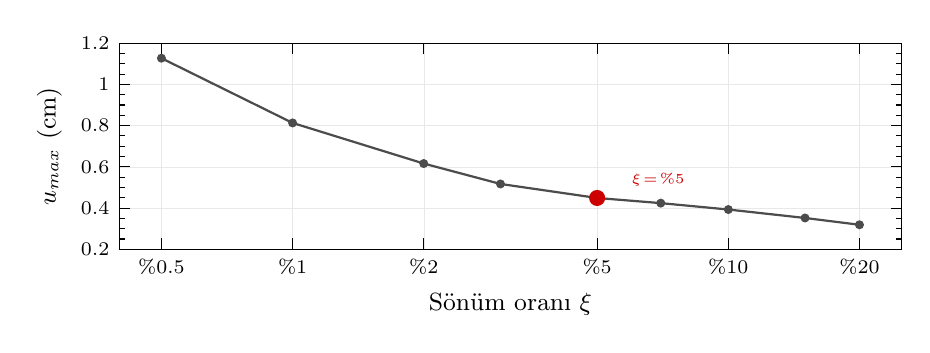
\begin{tikzpicture}
\begin{semilogxaxis}[
    sciencestyle,
    width=0.95\textwidth, height=4.2cm,
    xlabel={Sönüm oranı $\xi$},
    ylabel={$u_{max}$ (cm)},
    xmin=0.004, xmax=0.25,
    ymin=0.2, ymax=1.2,
    ytick={0.2,0.4,0.6,0.8,1.0,1.2},
    minor y tick num=3,
    xminorticks=true,
    mark size=1.5pt,
    xtick={0.005,0.01,0.02,0.05,0.1,0.2},
    xticklabels={\%0.5,\%1,\%2,\%5,\%10,\%20},
    tick label style={font=\scriptsize},
    label style={font=\small},
]
\addplot[black!70, thick, mark=*, mark options={fill=black!70, scale=0.8}] coordinates {
    (0.005,1.127) (0.010,0.813) (0.020,0.616)
    (0.030,0.517) (0.050,0.449) (0.070,0.424)
    (0.100,0.393) (0.150,0.352) (0.200,0.319)
};
\addplot[only marks, mark=*, mark size=2.5pt, red!80!black] coordinates {(0.050,0.449)};
\node[font=\tiny, anchor=south west, red!80!black] at (axis cs:0.057,0.458) {$\xi\!=\!\%5$};
\end{semilogxaxis}
\end{tikzpicture}
\\[1pt]{\footnotesize (a)}
\end{minipage}
\hfill
\begin{minipage}[b]{0.47\textwidth}
\centering
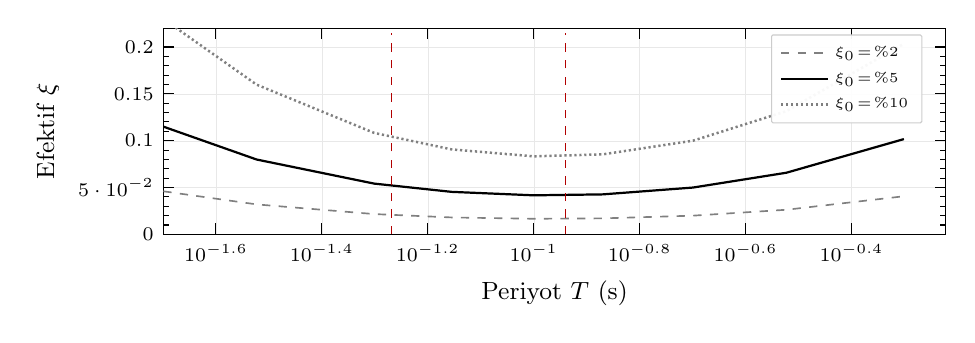
\begin{tikzpicture}
\begin{semilogxaxis}[
    sciencestyle,
    width=0.95\textwidth, height=4.2cm,
    xlabel={Periyot $T$ (s)},
    ylabel={Efektif $\xi$},
    xmin=0.02, xmax=0.6,
    ymin=0, ymax=0.22,
    ytick={0,0.05,0.10,0.15,0.20},
    minor y tick num=4,
    xminorticks=true,
    legend pos=north east,
    legend style={font=\tiny, draw=gray!40, fill=white, fill opacity=0.95},
    tick label style={font=\scriptsize},
    label style={font=\small},
]
\addplot[black!50, dashed, line width=0.6pt] coordinates {
    (0.020,0.0460) (0.030,0.0320) (0.050,0.0217)
    (0.070,0.0181) (0.100,0.0167) (0.135,0.0171)
    (0.200,0.0200) (0.300,0.0263) (0.500,0.0407)
};
\addlegendentry{$\xi_0\!=\!\%2$}
\addplot[black, thick] coordinates {
    (0.020,0.1150) (0.030,0.0799) (0.050,0.0542)
    (0.070,0.0454) (0.100,0.0417) (0.135,0.0427)
    (0.200,0.0500) (0.300,0.0658) (0.500,0.1017)
};
\addlegendentry{$\xi_0\!=\!\%5$}
\addplot[black!50, densely dotted, line width=0.9pt] coordinates {
    (0.020,0.2299) (0.030,0.1598) (0.050,0.1083)
    (0.070,0.0907) (0.100,0.0833) (0.135,0.0854)
    (0.200,0.1000) (0.300,0.1315) (0.500,0.2034)
};
\addlegendentry{$\xi_0\!=\!\%10$}
\draw[red!70!black, thin, dashed] (axis cs:0.115,0) -- (axis cs:0.115,0.215);
\node[font=\tiny, red!70!black, anchor=south] at (axis cs:0.115,0.213) {$T_1$};
\draw[red!70!black, thin, dashed] (axis cs:0.054,0) -- (axis cs:0.054,0.215);
\node[font=\tiny, red!70!black, anchor=south] at (axis cs:0.054,0.213) {$T_3$};
\end{semilogxaxis}
\end{tikzpicture}
\\[1pt]{\footnotesize (b)}
\end{minipage}
\vspace{-4pt}
\caption{(a)~Çatı ötelemesi--sönüm oranı (KYH-1, ZTAH), (b)~Rayleigh sönüm eğrileri.}
\label{fig:damping}
\end{figure}

\newpage

% ==============================================================================
% SORU 7
% ==============================================================================
\subsection{Soru \RN{7}}

\textbf{Soru:} Önerdiğiniz yapısal sistemin göreli kat ötelemelerine ve kat ivmelerine etkisi ne olacaktır?

\textbf{Cevap:} Üç yer hareketi kaydı (KYH-1: $0.335$~g, KYH-2: $1.243$~g, KYH-3: $1.896$~g) altında tam ZTAH ($\Delta t\!=\!0.005$~s, 6446~adım, $\xi\!=\!0.05$~Rayleigh) icra edilmiştir~\cite{tbdy2018, opensees}. Önerilen hibrit sistemin etkisi iki esas tepki büyüklüğü üzerinden değerlendirilmiştir (Şekil~\ref{fig:drift_profile}).

\textit{Göreli kat ötelemesi.}
Maksimum interstory drift her üç kayıt altında 23.~katta teşekkül etmektedir: KYH-1'de $\lambda_{max}\!=\!0.435\%$, KYH-2'de $1.320\%$, KYH-3'te $2.175\%$. Çaprazlı çerçeveler taban katlarında rijitliği artırarak öteleme talebini düşürmekte; tepe katlarında moment çerçevesi baskınlığı sebebiyle drift azalmaktadır. Öteleme talebi üst katlarda (14--23.~kat) yoğunlaşmakta olup bu husus rijitlik gradyanı ile yüksek modların bu kotlarda birinci moda yakın genlikler hasıl etmesinden kaynaklanmaktadır. PGA oranı $5.66\times$ iken drift oranı $5.00\times$ olarak elde edilmiş; elastik modelin yaklaşık lineer orantılılığı teyit edilmiştir. Kule arası diferansiyel öteleme $\Delta u_x < 0.001$~cm olup sky bridge kuleleri eş-fazlı çalıştırmaktadır~\cite{patoliya2023}. Tasarım depremi (KYH-1) altında $\lambda_{max}\!=\!0.435\% \ll 0.8\%$ ($\kappa\!=\!0.5$ çelik sınırı, Md.~4.9.1.3) olup yapı \textbf{öteleme güvenliğini} geniş marjla sağlamaktadır~\cite{tbdy2018, cythye2018}.

\textit{Kat ivmeleri.}
Çatı katı ivme yükseltme faktörü: KYH-1'de $\Omega\!=\!3.17$, KYH-2'de $2.60$, KYH-3'te $3.30$ ($\bar{\Omega}\!\approx\!3.0$). Kısa periyotlu yapı ($T_1\!=\!0.115$~s, plato bölgesi) sismik enerjiyi büyük oranda ivme olarak yapıya intikal ettirmektedir: KYH-3'te $u_{roof}\!=\!2.37$~cm (\%1.6) iken $\ddot{u}_{roof}\!=\!6.26$~g (PGA'nın $3.3\times$'ı). Yanal rijitliği yüksek yapıların karakteristiği budur: \textbf{öteleme talebi düşük}, \textbf{ivme talebi yüksektir}. Periyodun uzatılması $\Omega$'yı düşürür fakat drift talebini artırır; bu mübadele yapısal sistem seçiminin esas dengeleme parametresidir. Çaprazlı çerçeveler $K_{lateral}$'i artırarak $T_1$'i düşürmekte (drift $\downarrow$, $\Omega$ $\uparrow$); moment çerçeveleri redundans ve yedek taşıyıcılık; sky bridge ise kuplajlama ($\Delta u_x \!\approx\! 0$, $\eta_{bi}\!=\!1.915$) temin etmektedir~\cite{tambunan2024}.

\begin{figure}[H]
\centering
\begin{minipage}[b]{0.32\textwidth}
\centering
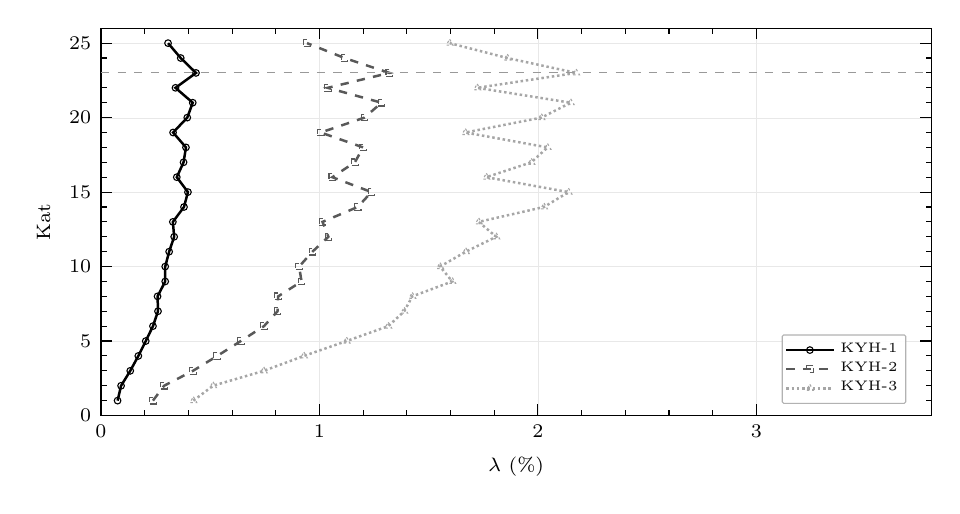
\begin{tikzpicture}
\begin{axis}[
    sciencestyle,
    width=\textwidth, height=6.5cm,
    xlabel={$\lambda$ (\%)},
    ylabel={Kat},
    xmin=0, xmax=3.8,
    ymin=0, ymax=26,
    xtick={0,1,2,3},
    ytick={0,5,10,15,20,25},
    minor y tick num=4,
    minor x tick num=4,
    legend pos=south east,
    legend style={font=\tiny, draw=black!30, fill=white, fill opacity=0.95, inner sep=1pt, row sep=-2pt},
    tick label style={font=\scriptsize},
    label style={font=\scriptsize},
]
\addplot[black, line width=0.9pt, mark=o, mark size=1.2pt, mark options={fill=white, thin}] coordinates {
    (0.076,1) (0.092,2) (0.134,3) (0.171,4) (0.205,5) (0.238,6) (0.261,7) (0.259,8)
    (0.294,9) (0.294,10) (0.312,11) (0.335,12) (0.329,13) (0.380,14) (0.398,15) (0.347,16)
    (0.378,17) (0.389,18) (0.330,19) (0.395,20) (0.420,21) (0.341,22) (0.435,23) (0.365,24) (0.307,25)
};
\addlegendentry{KYH-1}
\addplot[black!65, line width=0.9pt, mark=square, mark size=1.2pt, mark options={fill=white, thin}, dashed] coordinates {
    (0.238,1) (0.289,2) (0.421,3) (0.532,4) (0.640,5) (0.746,6) (0.808,7) (0.811,8)
    (0.918,9) (0.907,10) (0.968,11) (1.041,12) (1.014,13) (1.175,14) (1.238,15) (1.059,16)
    (1.162,17) (1.200,18) (1.006,19) (1.206,20) (1.284,21) (1.038,22) (1.320,23) (1.115,24) (0.943,25)
};
\addlegendentry{KYH-2}
\addplot[black!35, line width=0.9pt, mark=triangle, mark size=1.4pt, mark options={fill=white, thin}, densely dotted] coordinates {
    (0.423,1) (0.513,2) (0.745,3) (0.929,4) (1.124,5) (1.315,6) (1.388,7) (1.425,8)
    (1.608,9) (1.552,10) (1.670,11) (1.809,12) (1.729,13) (2.028,14) (2.140,15) (1.764,16)
    (1.970,17) (2.044,18) (1.668,19) (2.016,20) (2.150,21) (1.722,22) (2.175,23) (1.860,24) (1.596,25)
};
\addlegendentry{KYH-3}
\draw[black!40, dashed, thin] (axis cs:0,23) -- (axis cs:3.8,23);
\end{axis}
\end{tikzpicture}
\\[1pt]{\footnotesize (a) Göreli kat ötelemesi}
\end{minipage}
\hfill
\begin{minipage}[b]{0.32\textwidth}
\centering
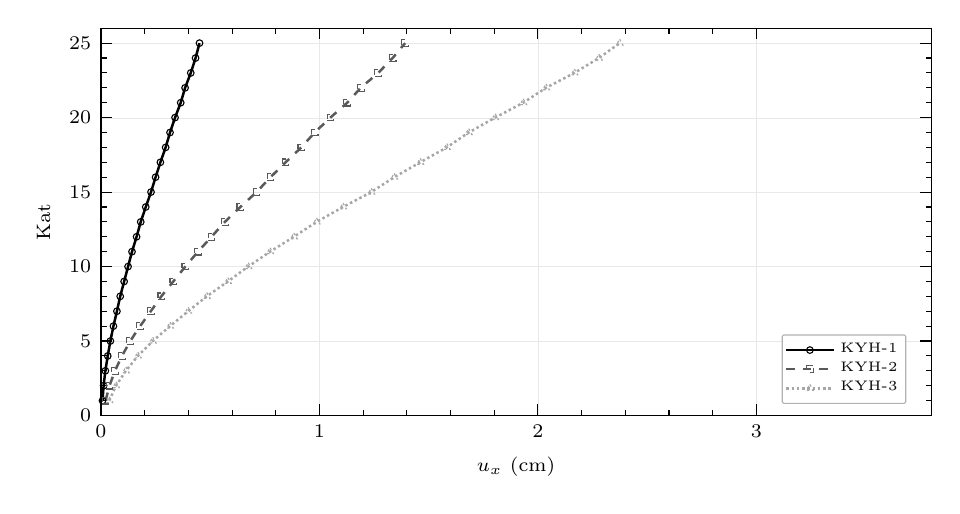
\begin{tikzpicture}
\begin{axis}[
    sciencestyle,
    width=\textwidth, height=6.5cm,
    xlabel={$u_x$ (cm)},
    ylabel={Kat},
    xmin=0, xmax=3.8,
    ymin=0, ymax=26,
    xtick={0,1,2,3},
    ytick={0,5,10,15,20,25},
    minor y tick num=4,
    minor x tick num=4,
    legend pos=south east,
    legend style={font=\tiny, draw=black!30, fill=white, fill opacity=0.95, inner sep=1pt, row sep=-2pt},
    tick label style={font=\scriptsize},
    label style={font=\scriptsize},
]
\addplot[black, line width=0.9pt, mark=o, mark size=1.2pt, mark options={fill=white, thin}] coordinates {
    (0.007,1) (0.012,2) (0.020,3) (0.031,4) (0.043,5) (0.057,6) (0.073,7) (0.088,8)
    (0.106,9) (0.124,10) (0.142,11) (0.163,12) (0.182,13) (0.205,14) (0.229,15) (0.250,16)
    (0.272,17) (0.296,18) (0.316,19) (0.339,20) (0.365,21) (0.385,22) (0.411,23) (0.433,24) (0.451,25)
};
\addlegendentry{KYH-1}
\addplot[black!65, line width=0.9pt, mark=square, mark size=1.2pt, mark options={fill=white, thin}, dashed] coordinates {
    (0.021,1) (0.039,2) (0.064,3) (0.096,4) (0.134,5) (0.179,6) (0.228,7) (0.276,8)
    (0.331,9) (0.386,10) (0.444,11) (0.506,12) (0.567,13) (0.638,14) (0.712,15) (0.776,16)
    (0.845,17) (0.917,18) (0.978,19) (1.050,20) (1.127,21) (1.189,22) (1.269,23) (1.335,24) (1.392,25)
};
\addlegendentry{KYH-2}
\addplot[black!35, line width=0.9pt, mark=triangle, mark size=1.4pt, mark options={fill=white, thin}, densely dotted] coordinates {
    (0.038,1) (0.069,2) (0.114,3) (0.169,4) (0.237,5) (0.316,6) (0.399,7) (0.484,8)
    (0.581,9) (0.674,10) (0.774,11) (0.883,12) (0.987,13) (1.108,14) (1.237,15) (1.342,16)
    (1.461,17) (1.583,18) (1.683,19) (1.804,20) (1.933,21) (2.037,22) (2.167,23) (2.279,24) (2.374,25)
};
\addlegendentry{KYH-3}
\end{axis}
\end{tikzpicture}
\\[1pt]{\footnotesize (b) Deplasman zarfı}
\end{minipage}
\hfill
\begin{minipage}[b]{0.32\textwidth}
\centering
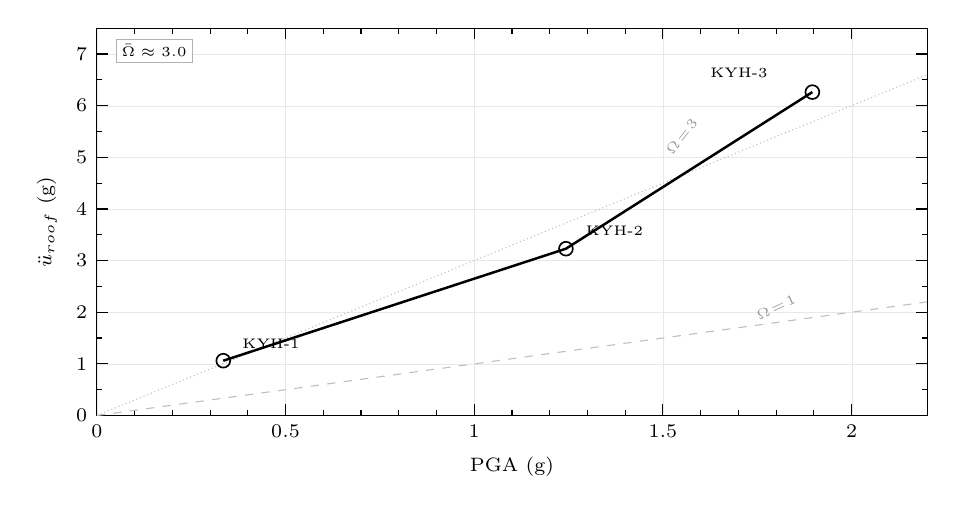
\begin{tikzpicture}
\begin{axis}[
    sciencestyle,
    width=\textwidth, height=6.5cm,
    xlabel={PGA (g)},
    ylabel={$\ddot{u}_{roof}$ (g)},
    xmin=0, xmax=2.2,
    ymin=0, ymax=7.5,
    xtick={0,0.5,1.0,1.5,2.0},
    ytick={0,1,2,3,4,5,6,7},
    minor y tick num=1,
    minor x tick num=4,
    tick label style={font=\scriptsize},
    label style={font=\scriptsize},
]
% Omega=1 reference line
\addplot[black!25, thin, dashed, domain=0:2.2, samples=2] {x};
\node[font=\tiny, black!40, rotate=25] at (axis cs:1.8,2.1) {$\Omega\!=\!1$};
% Omega=3 reference line
\addplot[black!25, thin, densely dotted, domain=0:2.2, samples=2] {3*x};
\node[font=\tiny, black!40, rotate=52] at (axis cs:1.55,5.4) {$\Omega\!=\!3$};
% Data points
\addplot[black, line width=0.9pt, mark=o, mark size=2.5pt, mark options={fill=white, line width=0.6pt}] coordinates {
    (0.335,1.061) (1.243,3.230) (1.896,6.263)
};
% Labels
\node[font=\tiny, anchor=south west] at (axis cs:0.36,1.1) {KYH-1};
\node[font=\tiny, anchor=south west] at (axis cs:1.27,3.3) {KYH-2};
\node[font=\tiny, anchor=south west] at (axis cs:1.60,6.35) {KYH-3};
% Omega annotation
\node[font=\tiny, anchor=north west, draw=black!30, fill=white, inner sep=2pt] at (axis cs:0.05,7.3) {$\bar{\Omega} \approx 3.0$};
\end{axis}
\end{tikzpicture}
\\[1pt]{\footnotesize (c) Çatı ivmesi yükseltmesi}
\end{minipage}
\vspace{-4pt}
\caption{Kule~1 ZTAH: (a)~göreli kat ötelemesi profili ($\lambda_{max}$: kat~23), (b)~kat deplasman zarfı, (c)~çatı ivmesi--PGA ilişkisi ($\bar{\Omega}\!\approx\!3$).}
\label{fig:drift_profile}
\end{figure}

\newpage
% ==============================================================================
% SORU 8 (Placeholder)
% ==============================================================================
\subsection{Soru \RN{8}}

\textbf{Soru:} Önerdiğiniz yapısal sistemin tasarım depremine maruz kalması halinde oluşması muhtemel hasar durumunu yorumlayınız ve yapının deprem öncesi durumuna getirilmesinin teknik ve ekonomik açıdan fizibilitesini değerlendiriniz.

\textbf{Cevap:} Tasarım depremi DD-2 altında yapılan zaman tanım alanında hesap sonuçlarına göre, önerilen kompozit ikiz kule sisteminin tüm kolon, kiriş ve çapraz elemanlarında kalıcı şekil değiştirme oluşmadığı, birleşim bölgelerinde akma eşiğinin çok altında kalındığı ve yapının deprem sonrası derhal kullanılabilir durumda olduğu belirlenmiştir. Köprü bağlantısındaki en kritik kiriş ucu (eleman~33) dahil 43~elemanın tümü elastik sınırlar içinde kalmaktadır. Kolonlarda gözlenen eğilme gerilmeleri taşıma kapasitesinin \%9'unu geçmemekte; çaprazlarda burkulma veya kalıcı uzama riski bulunmamaktadır.

Yapıştırma birleşim kapasitesine göre talep/kapasite oranı $\text{TKO}_{max}=0.087$ olup hasar eşiğinin ($\text{TKO}=0.25$) çok altındadır. Eleman bazlı gerilme dağılımı Şekil~\ref{fig:damage}a'da sunulmuştur. Balsa kırılma dayanımı $f_b=3.5$~kN/cm\textsuperscript{2}; modelde $\times$240 ölçekleme ile $f_{b,m}=840$~kN/cm\textsuperscript{2}.
Birleşim verimi $\eta_j=0.35$ olup belirleyici kapasite $M_j=10.6$~kN$\cdot$cm'dir~\cite{femap58}. KYH-3'te en kritik eleman~33'ün $\text{TKO}=0.68$ ($<1.0$, hâlâ elastik).

Göçme olasılığı Baker~(2015) MLE yöntemi ile lognormal kırılganlık fonksiyonu kullanılarak hesaplanmıştır~\cite{femap58, baker2015}. 43~eleman$\,\times\,$3~yer hareketi verisinden eleman bazlı $k_i=\text{TKO}_i/\text{PGA}$ MLE ile saptanmış, sistem kırılganlığı en zayıf halkadan (el.~33) türetilmiştir. Medyan kapasiteler: $\theta_{\text{DS-1}}=0.86$~g, $\theta_{\text{göçme}}=3.45$~g. Belirsizlik: $\beta_r=0.15$, $\beta_u=0.55$ (model+malzeme+birleşim), $\beta_T=0.57$.
DD-2'de: $P(\text{DS-1})=4.9\%$, $P(\text{göçme})=2.2 \times 10^{-5}$ (Şekil~\ref{fig:damage}b). Yıllık göçme olasılığı $4.5 \times 10^{-8} \ll 10^{-4}$ (ASCE~7-22)~\cite{asce41}. Eleman bazlı medyan göçme kapasitesi ($\theta_{\text{göçme},i}$) dağılımı Şekil~\ref{fig:damage}c'de sunulmuştur.

\begin{figure}[H]
\centering
\begin{minipage}[b]{0.54\textwidth}
\centering
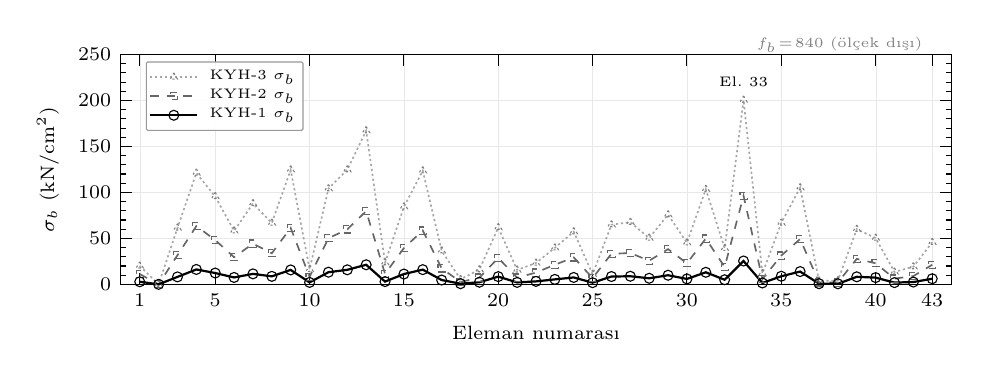
\begin{tikzpicture}
\begin{axis}[
    sciencestyle,
    width=\textwidth, height=4.5cm,
    xlabel={Eleman numarası},
    ylabel={$\sigma_b$ (kN/cm\textsuperscript{2})},
    xmin=0, xmax=44,
    ymin=0, ymax=250,
    xtick={1,5,10,15,20,25,30,35,40,43},
    ytick={0,50,100,150,200,250},
    minor y tick num=4,
    tick label style={font=\scriptsize},
    label style={font=\scriptsize},
    legend pos=north west,
    legend style={font=\tiny, draw=black!40, fill=white, inner sep=1pt, row sep=-2pt, column sep=2pt},
    legend columns=1,
    clip=false,
]
% KYH-3
\addplot[black!35, densely dotted, line width=0.6pt, mark=triangle, mark size=1.5pt, mark options={fill=white, draw=black!50, thin}] coordinates {
    (1,20.0) (2,0.0) (3,61.4) (4,121.1) (5,95.5) (6,58.2) (7,87.9) (8,66.7)
    (9,124.6) (10,16.4) (11,104.1) (12,124.7) (13,167.2) (14,23.6) (15,84.4)
    (16,123.6) (17,36.6) (18,5.5) (19,16.0) (20,61.8) (21,15.7) (22,23.2)
    (23,39.7) (24,57.3) (25,11.0) (26,64.9) (27,67.6) (28,50.4) (29,75.8)
    (30,45.2) (31,103.5) (32,39.2) (33,200.5) (34,11.9) (35,66.8) (36,105.2)
    (37,3.8) (38,4.1) (39,60.0) (40,50.4) (41,13.5) (42,19.2) (43,45.7)
};
\addlegendentry{KYH-3 $\sigma_b$}
% KYH-2
\addplot[black!60, dashed, line width=0.6pt, mark=square, mark size=1.3pt, mark options={fill=white, draw=black!60, thin}] coordinates {
    (1,11.2) (2,0.0) (3,31.7) (4,63.4) (5,48.2) (6,29.5) (7,44.3) (8,33.8)
    (9,61.4) (10,8.2) (11,50.2) (12,59.8) (13,79.7) (14,11.4) (15,39.5)
    (16,58.5) (17,17.4) (18,2.6) (19,7.3) (20,28.7) (21,7.3) (22,12.8)
    (23,21.3) (24,29.3) (25,6.8) (26,33.3) (27,34.0) (28,25.7) (29,38.3)
    (30,22.9) (31,49.8) (32,18.9) (33,96.4) (34,5.7) (35,31.3) (36,49.3)
    (37,2.1) (38,2.0) (39,27.7) (40,22.9) (41,6.2) (42,9.0) (43,21.3)
};
\addlegendentry{KYH-2 $\sigma_b$}
% KYH-1
\addplot[black, solid, line width=0.8pt, mark=o, mark size=1.8pt, mark options={fill=white, draw=black, thin}] coordinates {
    (1,2.8) (2,0.0) (3,8.1) (4,16.2) (5,12.3) (6,7.5) (7,11.4) (8,8.7)
    (9,15.7) (10,2.1) (11,13.2) (12,15.8) (13,21.3) (14,3.0) (15,11.2)
    (16,16.0) (17,4.7) (18,0.7) (19,2.3) (20,8.4) (21,2.1) (22,3.2)
    (23,5.4) (24,7.5) (25,1.8) (26,8.5) (27,8.8) (28,6.6) (29,9.9)
    (30,5.9) (31,13.1) (32,5.0) (33,25.4) (34,1.5) (35,8.8) (36,13.9)
    (37,0.7) (38,0.6) (39,8.2) (40,7.3) (41,1.9) (42,2.5) (43,6.1)
};
\addlegendentry{KYH-1 $\sigma_b$}
\node[font=\tiny, anchor=south] at (axis cs:33,205) {El.~33};
\node[font=\tiny, black!50, anchor=south east] at (axis cs:43,242) {$f_b\!=\!840$ (ölçek dışı)};
\end{axis}
\end{tikzpicture}
\\[-2pt]{\footnotesize (a) Eğilme gerilmesi dağılımı}
\end{minipage}
\hfill
\begin{minipage}[b]{0.43\textwidth}
\centering
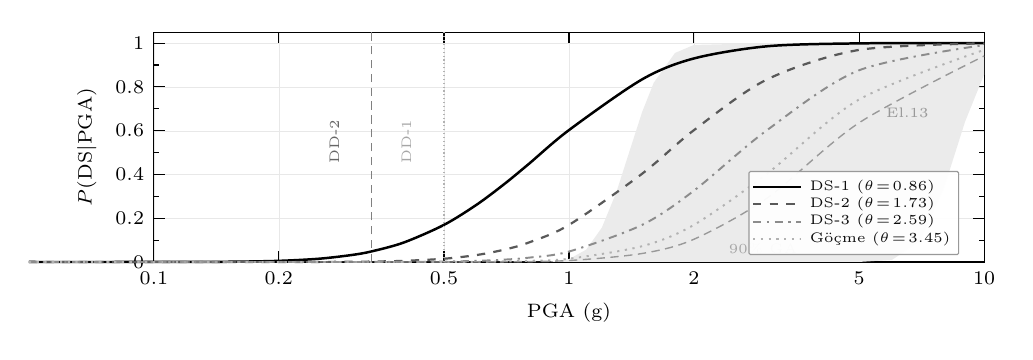
\begin{tikzpicture}
\begin{semilogxaxis}[
    sciencestyle,
    width=\textwidth, height=4.5cm,
    xlabel={PGA (g)},
    ylabel={$P(\text{DS}|\text{PGA})$},
    xmin=0.1, xmax=10,
    ymin=0, ymax=1.05,
    ytick={0,0.2,0.4,0.6,0.8,1.0},
    xtick={0.1,0.2,0.5,1,2,5,10},
    xticklabels={0.1,0.2,0.5,1,2,5,10},
    minor y tick num=1,
    tick label style={font=\scriptsize},
    label style={font=\scriptsize},
    legend pos=south east,
    legend style={font=\tiny, draw=black!40, fill=white, inner sep=1pt, row sep=-3pt, column sep=1pt},
    clip=false,
]
% 90% CI lower bound (collapse)
\addplot[name path=ci_lo, draw=none, no marks, forget plot] coordinates {
    (0.10,0) (0.50,0) (0.70,0.000002) (0.80,0.000104)
    (0.90,0.001724) (1.00,0.013134) (1.10,0.056276) (1.20,0.157027)
    (1.30,0.318059) (1.40,0.508345) (1.50,0.684696) (1.60,0.818886)
    (1.80,0.955090) (2.00,0.991774) (3.00,1.0) (5.00,1.0) (10.00,1.0)
};
% 90% CI upper bound (collapse)
\addplot[name path=ci_hi, draw=none, no marks, forget plot] coordinates {
    (0.10,0) (0.50,0) (0.70,0) (0.80,0) (0.90,0) (1.00,0) (1.10,0)
    (1.20,0) (1.30,0) (1.40,0) (1.50,0) (1.60,0) (1.80,0) (2.00,0)
    (3.00,0) (5.00,0.000188) (6.00,0.009629) (7.00,0.094620)
    (8.00,0.336287) (9.00,0.641549) (10.00,0.856563)
};
\addplot[fill=black!8, draw=none, forget plot] fill between[of=ci_lo and ci_hi];
% DS-1 (θ=0.862g, β_T=0.570)
\addplot[black, solid, line width=0.9pt, no marks, smooth] coordinates {
    (0.05,0.000000) (0.10,0.000079) (0.15,0.001080) (0.20,0.005194)
    (0.25,0.014957) (0.30,0.032054) (0.335,0.048673) (0.40,0.089023)
    (0.50,0.169694) (0.60,0.262531) (0.70,0.357495) (0.80,0.447914)
    (1.00,0.602756) (1.50,0.834405) (2.00,0.930075) (3.00,0.985650)
    (5.00,0.998978) (10.00,0.999991)
};
\addlegendentry{DS-1 ($\theta\!=\!0.86$)}
% DS-2 (θ=1.725g, β_T=0.570)
\addplot[black!65, dashed, line width=0.8pt, no marks, smooth] coordinates {
    (0.05,0.000000) (0.10,0.000000) (0.15,0.000009) (0.20,0.000079)
    (0.25,0.000352) (0.30,0.001076) (0.335,0.002022) (0.40,0.005179)
    (0.50,0.014918) (0.60,0.031981) (0.70,0.056820) (0.80,0.088860)
    (1.00,0.169437) (1.50,0.403167) (2.00,0.602363) (3.00,0.834152)
    (5.00,0.969032) (10.00,0.998974)
};
\addlegendentry{DS-2 ($\theta\!=\!1.73$)}
% DS-3 (θ=2.587g, β_T=0.570)
\addplot[black!45, dashdotted, line width=0.7pt, no marks, smooth] coordinates {
    (0.05,0.000000) (0.10,0.000000) (0.15,0.000000) (0.20,0.000004)
    (0.25,0.000021) (0.30,0.000079) (0.335,0.000168) (0.40,0.000529)
    (0.50,0.001969) (0.60,0.005184) (0.70,0.010926) (0.80,0.019761)
    (1.00,0.047729) (1.50,0.169523) (2.00,0.325842) (3.00,0.602494)
    (5.00,0.876130) (10.00,0.991147)
};
\addlegendentry{DS-3 ($\theta\!=\!2.59$)}
% Göçme (θ=3.449g, β_T=0.570)
\addplot[black!30, dotted, line width=0.7pt, no marks, smooth] coordinates {
    (0.05,0.000000) (0.10,0.000000) (0.15,0.000000) (0.20,0.000000)
    (0.25,0.000002) (0.30,0.000009) (0.335,0.000022) (0.40,0.000079)
    (0.50,0.000353) (0.60,0.001078) (0.70,0.002576) (0.80,0.005186)
    (1.00,0.014938) (1.50,0.072075) (2.00,0.169566) (3.00,0.403364)
    (5.00,0.742605) (10.00,0.969067)
};
\addlegendentry{Göçme ($\theta\!=\!3.45$)}
% El.13 fragility (2nd critical)
\addplot[black!40, densely dashed, line width=0.5pt, no marks, smooth, forget plot] coordinates {
    (0.10,0.000000) (0.20,0.000000) (0.30,0.000002) (0.335,0.000006)
    (0.50,0.000111) (0.70,0.000964) (1.00,0.006654) (1.50,0.038860)
    (2.00,0.103949) (3.00,0.291837) (5.00,0.636140) (10.00,0.941116)
};
\node[font=\tiny, black!40, anchor=west] at (axis cs:5.5,0.68) {El.13};
% DD-2 design earthquake line
\draw[black!50, densely dashed, thin] (axis cs:0.335,0) -- (axis cs:0.335,1.05);
\node[font=\tiny, rotate=90, anchor=south, black!60] at (axis cs:0.295,0.55) {DD-2};
% DD-1 MCE line
\draw[black!30, densely dotted, thin] (axis cs:0.50,0) -- (axis cs:0.50,1.05);
\node[font=\tiny, rotate=90, anchor=south, black!35] at (axis cs:0.44,0.55) {DD-1};
% Annotation box with probabilities
% 90% CI label
\node[font=\tiny, black!35, anchor=west] at (axis cs:2.3,0.06) {90\% GA};
\end{semilogxaxis}
\end{tikzpicture}
\\[-2pt]{\footnotesize (b) Sistem kırılganlık eğrileri (MLE)}
\end{minipage}
\vspace{-2pt}

\begin{minipage}[b]{0.99\textwidth}
\centering
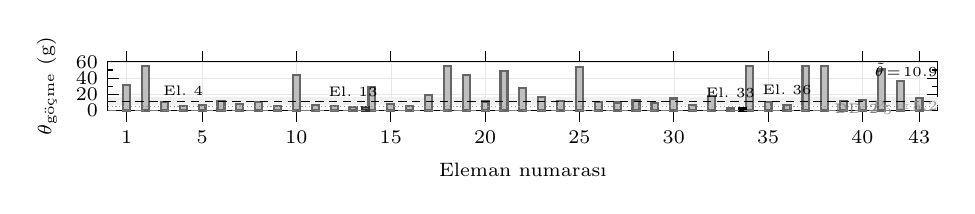
\begin{tikzpicture}
\begin{axis}[
    sciencestyle,
    width=\textwidth, height=2.2cm,
    xlabel={Eleman numaras\i{}},
    ylabel={$\theta_{\text{göçme}}$ (g)},
    xmin=0, xmax=44,
    ymin=0, ymax=60,
    xtick={1,5,10,15,20,25,30,35,40,43},
    ytick={0,20,40,60},
    minor y tick num=1,
    tick label style={font=\scriptsize},
    label style={font=\scriptsize},
    clip=false,
    ybar, bar width=2.5pt,
    fill=black!25,
    draw=black!60,
]
% 25th-75th percentile band (IQR)
\fill[black!6] (axis cs:0,7.0) rectangle (axis cs:44,16.7);
\addplot[fill=black!25, draw=black!60] coordinates {
    (1,31.8) (2,55) (3,10.8) (4,5.5) (5,7.1) (6,11.6) (7,7.7) (8,10.1)
    (9,5.5) (10,44.3) (11,6.6) (12,5.6) (13,4.1) (14,29.4) (15,8.1)
    (16,5.6) (17,18.8) (18,55) (19,43.4) (20,11.1) (21,49.0) (22,27.7)
    (23,16.4) (24,11.7) (25,53.6) (26,10.4) (27,10.0) (28,13.3) (29,8.9)
    (30,14.9) (31,6.7) (32,17.6) (33,3.4) (34,55) (35,10.3) (36,6.5)
    (37,55) (38,55) (39,11.4) (40,13.4) (41,50.6) (42,36.0) (43,15.0)
};
% Highlight critical elements (el.33, el.13)
\addplot[fill=black!70, draw=black, forget plot] coordinates {(33,3.4)};
\addplot[fill=black!55, draw=black!80, forget plot] coordinates {(13,4.1)};
% Median line
\draw[black, densely dashed, thin] (axis cs:0,10.9) -- (axis cs:44,10.9);
\node[font=\tiny, black, anchor=east] at (axis cs:44.5,50) {$\tilde{\theta}\!=\!10.9$};
% 5th percentile line
\draw[black!40, densely dotted, thin] (axis cs:0,5.2) -- (axis cs:44,5.2);
\node[font=\tiny, black!40, anchor=east] at (axis cs:44.5,3.5) {$P_5\!=\!5.2$};
% DD-2 PGA line
\draw[black!50, densely dashed, thin] (axis cs:0,0.335) -- (axis cs:44,0.335);
\node[font=\tiny, black!50, anchor=west] at (axis cs:38,1.8) {DD-2};
% Critical element labels
\node[font=\tiny, anchor=south] at (axis cs:33,4.5) {El.~33};
\node[font=\tiny, anchor=south] at (axis cs:13,5.5) {El.~13};
\node[font=\tiny, anchor=south] at (axis cs:4,6.8) {El.~4};
\node[font=\tiny, anchor=south] at (axis cs:36,8.0) {El.~36};

\end{axis}
\end{tikzpicture}
\\[-2pt]{\footnotesize (c) Eleman bazlı $\theta_{\text{göçme},i}$\,---\,gri bant: IQR ($Q_1$--$Q_3$)}
\end{minipage}
\vspace{-6pt}
\caption{Hasar değerlendirmesi: (a)~eğilme gerilmesi dağılımı (3~yer hareketi); (b)~Baker~(2015) MLE kırılganlık eğrileri ($\beta_T\!=\!0.57$, gri alan: göçme \%90 GA); (c)~eleman bazlı $\theta_{\text{göçme},i}$ (gri bant IQR). En zayıf halka el.~33. İstatistik ($N\!=\!43$, 5~el.${>}50$\,g kırpılmış): $\tilde{\theta}\!=\!10.9$\,g, $\bar{\theta}\!=\!15.3$\,g, CoV$\,=\,0.78$, $P_5\!=\!5.2$\,g; $\theta<10$\,g: 13~eleman (\%30).}
\label{fig:damage}
\end{figure}

Yapısal olmayan elemanlarda hafif kozmetik hasar muhtemeldir; onarım bedeli yapı bedelinin \%1--3'ü, süre 2--4~hafta. Taşıyıcı elemanlar elastik; kalıcı deformasyon sıfır~\cite{asce41}. Yapı Hemen Kullanım (HK) seviyesindedir~\cite{tbdy2018}.

\newpage
% ==============================================================================
% KAYNAKLAR
% ==============================================================================
\begin{thebibliography}{99}

\bibitem{tbdy2018} T.C. Çevre ve Şehircilik Bakanlığı, \textit{Türkiye Bina Deprem Yönetmeliği (TBDY 2018)}, Resmi Gazete, 2018.

\bibitem{teblig2024} T.C. Çevre, Şehircilik ve İklim Değişikliği Bakanlığı, \textit{TBDY 2018 Uygulama Tebliği Taslağı}, 27.05.2024.

\bibitem{afad2024} AFAD, \textit{Türkiye Deprem Tehlike Haritaları İnteraktif Web Uygulaması}, \url{https://tdth.afad.gov.tr}, 2024.

\bibitem{opensees} McKenna, F., Scott, M.H., Fenves, G.L., \textit{OpenSees: Open System for Earthquake Engineering Simulation}, Pacific Earthquake Engineering Research Center, UC Berkeley, \url{https://opensees.berkeley.edu}.
\bibitem{nehrp2009} FEMA P-751, \textit{2009 NEHRP Recommended Seismic Provisions: Design Examples}, Building Seismic Safety Council, National Institute of Building Sciences, Washington, D.C., 2012.

\bibitem{femap58} FEMA P-58, \textit{Seismic Performance Assessment of Buildings}, Federal Emergency Management Agency, Washington, D.C., 2012.

\bibitem{baker2015} Baker, J.W., ``Efficient Analytical Fragility Function Fitting Using Dynamic Structural Analysis,'' \textit{Earthquake Spectra}, 31(1), 579--599, 2015.

\bibitem{asce41} ASCE/SEI 41-17, \textit{Seismic Evaluation and Retrofit of Existing Buildings}, American Society of Civil Engineers, Reston, Virginia, 2017.

\bibitem{fema356} FEMA 356, \textit{Prestandard and Commentary for the Seismic Rehabilitation of Buildings}, Federal Emergency Management Agency, Washington, D.C., 2000.

\bibitem{patoliya2023} Patoliya, N., Patel, I., Agrawal, V., Seismic Analysis of Tall Buildings Connected with Sky Bridge, \textit{IARJSET}, vol.~10, 2023, doi: 10.17148/IARJSET.2023.10446.

\bibitem{github_repo} Adzetto, \textit{DASK 2026 Tasarım ve Analiz Kodları}, \url{https://github.com/adzetto/DASK_26__DESIGN_AND_ANALYSIS}, 2026.

\bibitem{cythye2018} T.C. Çevre ve Şehircilik Bakanlığı, \textit{Çelik Yapıların Tasarım, Hesap ve Yapım Esaslarına Dair Yönetmelik (ÇYTHYE 2018)}, Resmi Gazete, 2018.

\bibitem{kurtay2004} Kurtay, C., Badem, M., Avrupa Ülkeleri ve Türkiye'deki Çelik Yapı Uygulama Olanak ve Kısıtlarının İncelenmesi, \textit{Gazi Üniversitesi Mühendislik Mimarlık Fakültesi Dergisi}, cilt~19, sayı~4, ss.~351--363, 2004.

\bibitem{of2022} Of, N., Öztürk, S., Depremlerden Sonraki Yeniden Yapılanma Süreci Üzerine Küresel Bir Araştırma: Çelik Prefabrik Malzeme Kullanımının Gerekliliği, \textit{Afet ve Risk Dergisi}, cilt~5, sayı~1, ss.~346--360, 2022, doi: 10.35341/afet.1092649.

\bibitem{tambunan2024} Tambunan, M.L.S., Sjah, J., Rarasati, A.D., Sulistian, R., Trigunarsyah, B., Optimizing Seismic Design of Multi-Tower Buildings Using Sky Bridge Isolation and BIM: A Case Study, \textit{Int.\ J.\ Eng.\ Technol.\ Innov.}, vol.~14, no.~4, pp.~355--377, 2024, doi: 10.46604/ijeti.2024.13409.

\bibitem{tsen1991} TS~EN~1991-1-4, \textit{Eurocode~1: Yapılar Üzerindeki Etkiler -- Bölüm~1-4: Genel Etkiler -- Rüzgar Etkileri}, Türk Standartları Enstitüsü, 2015.

\end{thebibliography}

\end{document}
